\documentclass[11pt]{article}
\usepackage[a4paper, margin=2.5cm]{geometry}
\usepackage{graphicx}
\usepackage{caption}
\usepackage{pdfcomment}
\usepackage{float}
\usepackage{tikz}
\usepackage[polish]{babel}
\usepackage[utf8]{inputenc}
\usepackage[T1]{fontenc}
\captionsetup{font=small, skip=6pt}
\usepackage{titlesec}
\usepackage{parskip}
\setlength{\parskip}{4pt}
\setlength{\textfloatsep}{10pt}
\setlength{\floatsep}{6pt}
\setlength{\intextsep}{10pt}

\titlespacing*{\section}{0pt}{2ex plus .2ex minus .2ex}{1ex plus .2ex}
\titlespacing*{\subsection}{0pt}{1ex plus .1ex minus .1ex}{0.5ex plus .1ex}

    
\usepackage{parskip}
\setlength{\parskip}{2pt}

\title{Wzmacniacze mocy w napędzie elektrycznym. Przekształtnik tranzystorowy i tyrystorowy.}

\author{
  Mateusz Jaworski \\
  Piotr Migdałek \\
  Paweł Michalski \\
  Jakub Jaszczak \\
  Franciszek Janicki
}

\begin{document}

\maketitle

\tableofcontents
\newpage

\section{Część I}

\subsection{WZMACNIACZ LINIOWY / WZMACNIACZ IMPULSOWY}

a) Badanie sprawności wzmacniacza liniowego BJT

Zbadano moc na wejściu i wyjściu wzmacniacza liniowego w technologii BJT.\\

\begin{figure}[H]
\centering
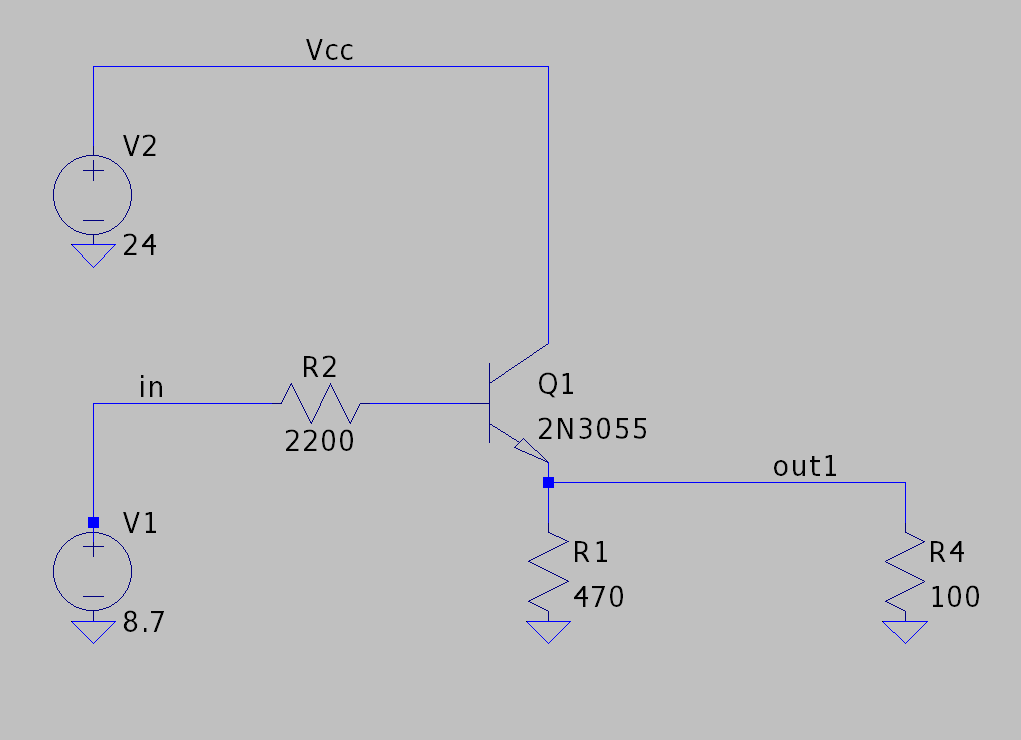
\includegraphics[width=0.8\textwidth]{aun1_liniowy_bjt.png}
\caption{Schemat pomiarowy wzmacniacza liniowego BJT}
\end{figure}

\begin{table}[H]
\centering
\begin{tabular}{|c|c|c|c|c|}
\hline
\textbf{Vcc [V]} & \textbf{V\_in [V]} & \textbf{P\_in + P\_vcc [mW]} & \textbf{P\_out [W]} & \textbf{Sprawność [\%]} \\
\hline
24 & 2  & 0{,}667  & 0{,}014683 & 2{,}201 \\
\hline
24 & 4  & 1{,}525  & 0{,}070000 & 4{,}590 \\
\hline
24 & 6  & 2{,}380  & 0{,}166000 & 6{,}975 \\
\hline
24 & 8  & 3{,}242  & 0{,}360000 & 11{,}104 \\
\hline
24 & 10 & 4{,}097  & 0{,}477000 & 11{,}643 \\
\hline
24 & 12 & 4{,}950  & 0{,}690000 & 13{,}939 \\
\hline
24 & 14 & 5{,}800  & 0{,}941000 & 16{,}224 \\
\hline
24 & 16 & 6{,}640  & 1{,}220000 & 18{,}373 \\
\hline
24 & 18 & 7{,}490  & 1{,}540000 & 20{,}561 \\
\hline
24 & 20 & 8{,}330  & 1{,}940000 & 23{,}289 \\
\hline
\end{tabular}
\caption{Sprawność pracy wzmacniacza liniowego BJT}
\end{table}

Jak widzimy sprawność jest bardzo mała. Wynika to z faktu, że tranzystor nie wysterowuje się całkowicie,
część energii przekształcana jest na ciepło.

b) Badanie sprawności wzmacniacza impulsowego BJT, porównanie z wzmacniaczem liniowym BJT

Zbadano moc na wejściu i wyjściu wzmacniacza impulsowego w technologii BJT.\\

\begin{figure}[H]
\centering
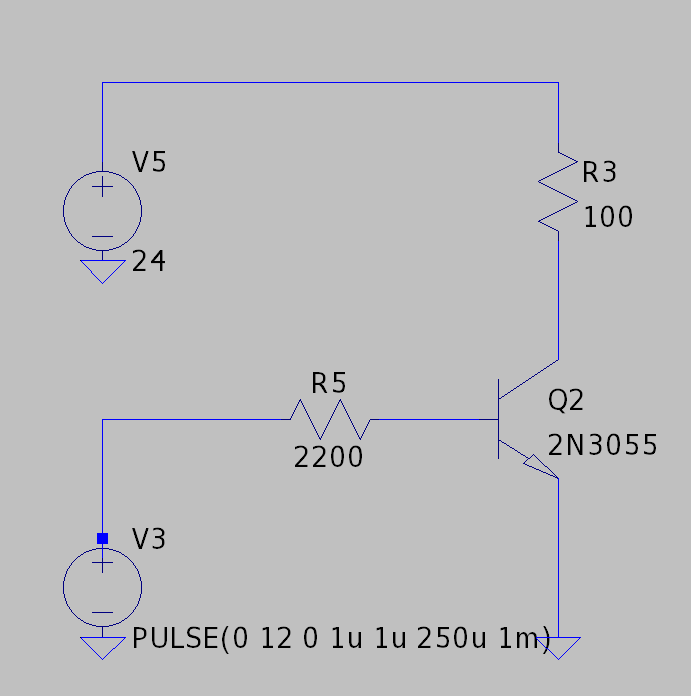
\includegraphics[width=0.8\textwidth]{aun1_impulsowy_bjt.png}
\caption{Schemat pomiarowy wzmacniacza impulsowego BJT}
\end{figure}

\begin{table}[H]
\centering
\begin{tabular}{|c|c|c|c|c|}
\hline
\textbf{Vcc [V]} & \textbf{V\_in [V]} & \textbf{P\_vcc + P\_in [W]} & \textbf{P\_out [W]} & \textbf{Sprawność [\%]} \\
\hline
24 & 2  & 0{,}54825 & 0{,}499   & 91{,}017 \\
\hline
24 & 4  & 1{,}054   & 0{,}974   & 92{,}410 \\
\hline
24 & 6  & 1{,}549   & 1{,}453   & 93{,}802 \\
\hline
24 & 8  & 2{,}046   & 1{,}928   & 94{,}233 \\
\hline
24 & 10 & 2{,}544   & 2{,}4023  & 94{,}430 \\
\hline
24 & 12 & 3{,}0476  & 2{,}882   & 94{,}566 \\
\hline
24 & 14 & 3{,}545   & 3{,}356   & 94{,}669 \\
\hline
24 & 16 & 4{,}042   & 3{,}831   & 94{,}780 \\
\hline
24 & 18 & 4{,}546   & 4{,}311   & 94{,}831 \\
\hline
24 & 20 & 5{,}043   & 4{,}833   & 95{,}836 \\
\hline
\end{tabular}
\caption{Sprawność pracy wzmacniacza impulsowego BJT}
\end{table}

Jak widzimy, sprawność jest bardzo duża, wynika to z faktu, że wzmacniacz impulsowy działa tylko w 2 stanach tranzystora:
zaporowym oraz przewodzenia, gdzie kiedy klucz jest rozłączony, nie ma strat, w momencie przewodzenia straty są minimalne. Przy dużych częstotliwościach przełączania główne źródło strat to straty łączeniowe, które możemy minimalizować dobierając tranzystor o odpowiednich parametrach.\\

Porównano sprawności wzmacniaczy liniowego oraz impulsowego w technologii BJT.\\

\begin{figure}[H]
\centering
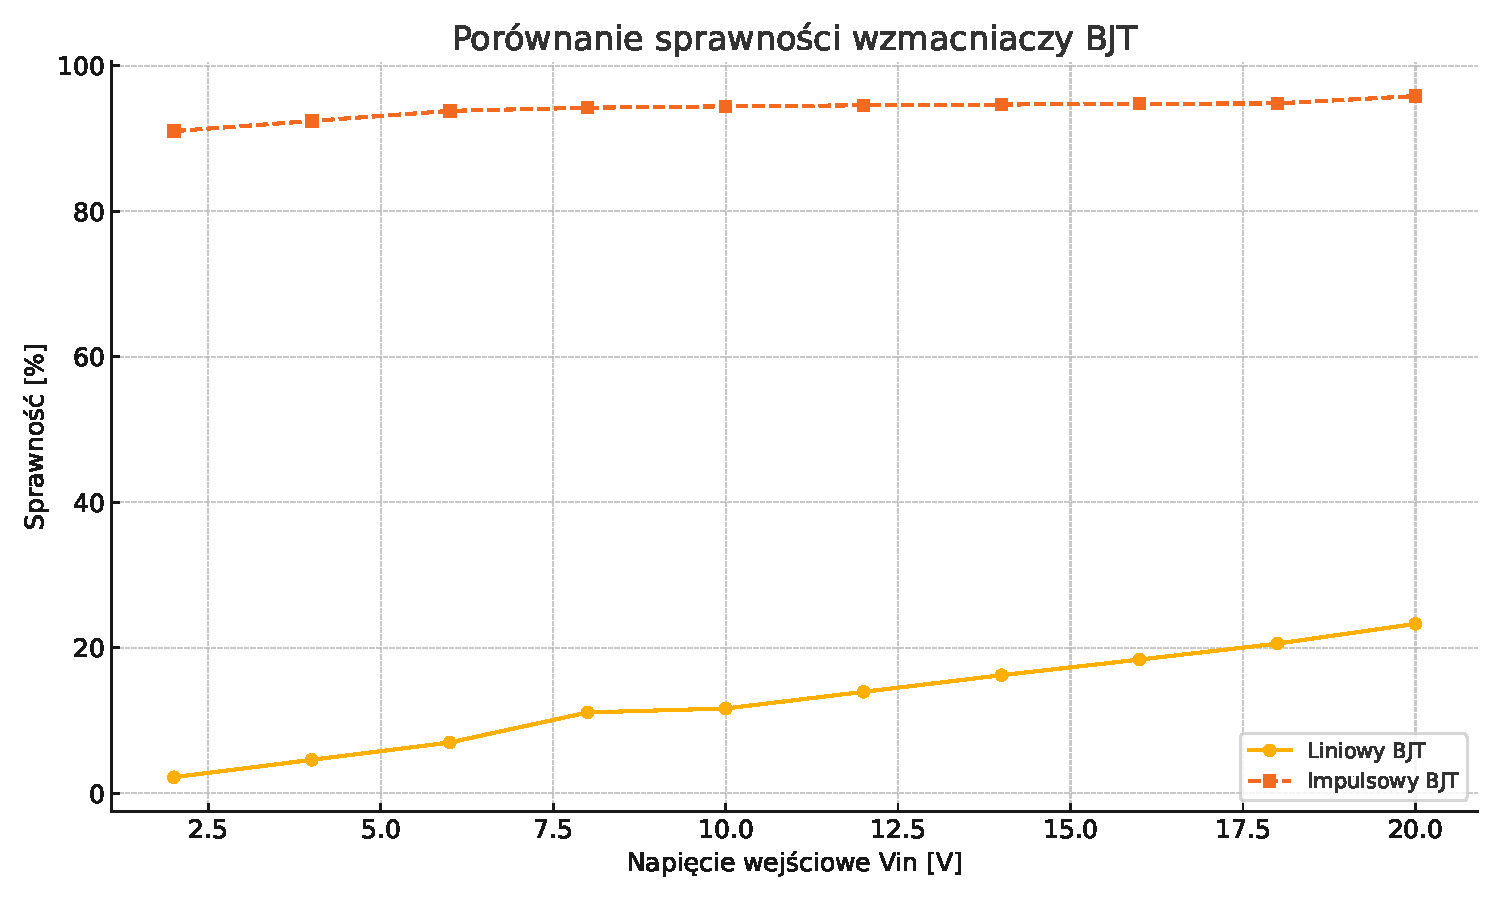
\includegraphics[width=0.8\textwidth]{aun1_liniowy_impulsowy_bjt.pdf}
\caption{Wykres sprawności wzmacniacza liniowego i impulsowego BJT}
\end{figure}

Jak widzimy, w obydwu przypadkach sprawność rośnie wraz ze zbliżaniem się napięcia średniego na tranzystorze do napięcia zasilania. Wzmacniacz impulsowy który zachowuje bardzo dużą sprawność dla całego zakresu napięcia ma znacząca przewagę,
wykorzystuje bowiem jedynie stan przewodzenia i zaporowy, a jedyne znaczące straty to straty łączeniowe
(straty przewodzenia odgrywają dużą rolę tylko przy niższych częstotliwościach).\\

\subsection{TECHNOLOGIA BJT/MOSFET}

c) Badanie sprawności wzmacniacza impulsowego MOSFET i porównanie z wzmacniaczem impulsowym BJT oraz porównanie wpływu Rds_on i ładunku bramki na sprawność

Zbadano moc na wejściu i wyjściu wzmacniacza impulsowego w technologiach BJT i MOSFET.\\

\begin{figure}[H]
\centering
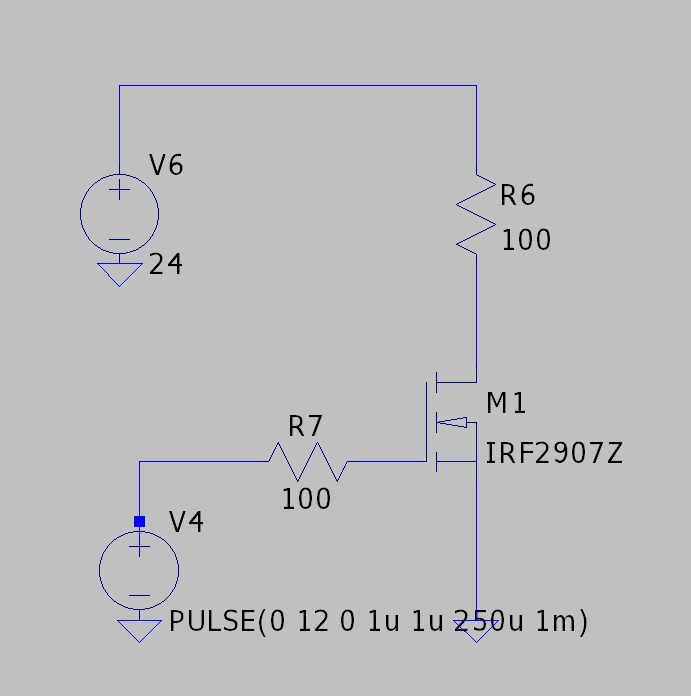
\includegraphics[width=0.8\textwidth]{aun1_impulsowy_mosfet.png}
\caption{Schemat pomiarowy wzmacniacza impulsowego MOSFET}
\end{figure}

\begin{table}[H]
\centering
\begin{tabular}{|c|c|c|c|c|}
\hline
\textbf{Vcc [V]} & \textbf{V\_in [V]} & \textbf{P\_vcc + P\_in [mW]} & \textbf{P\_out [W]} & \textbf{Sprawność [\%]} \\
\hline
24 & 2  & 0{,}499    & 0{,}4956   & 99{,}319 \\
\hline
24 & 4  & 0{,}95412  & 0{,}9506   & 99{,}631 \\
\hline
24 & 6  & 1{,}461    & 1{,}4575   & 99{,}760 \\
\hline
24 & 8  & 1{,}939    & 1{,}9355   & 99{,}819 \\
\hline
24 & 10 & 2{,}417    & 2{,}4135   & 99{,}855 \\
\hline
24 & 12 & 2{,}9009   & 2{,}8974   & 99{,}879 \\
\hline
24 & 14 & 3{,}379    & 3{,}375    & 99{,}882 \\
\hline
24 & 16 & 3{,}857    & 3{,}853    & 99{,}896 \\
\hline
24 & 18 & 4{,}3409   & 4{,}3373   & 99{,}917 \\
\hline
24 & 20 & 5{,}760    & 5{,}759    & 99{,}983 \\
\hline
\end{tabular}
\caption{Sprawność pracy wzmacniacza impulsowego MOSFET}
\end{table}

\begin{figure}[H]
\centering
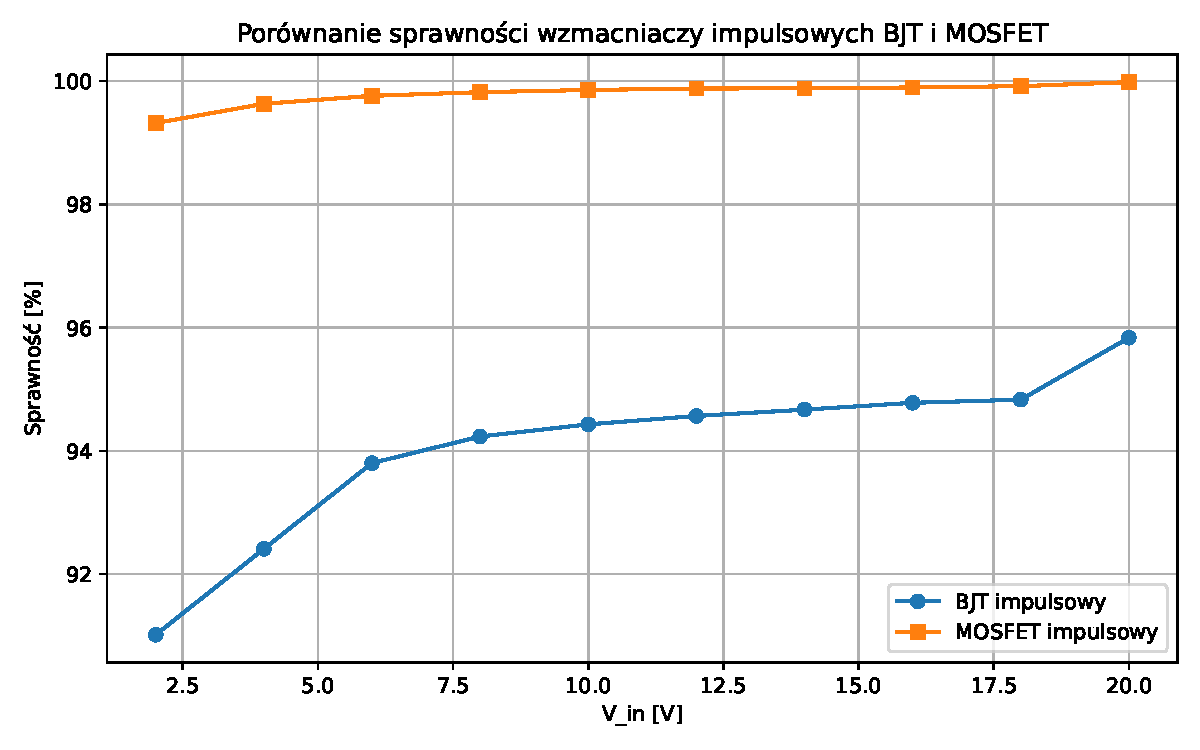
\includegraphics[width=0.8\textwidth]{aun1_imp_bjt_vs_mosfet.pdf}
\caption{Wykres sprawności wzmacniacza impulsowego BJT i MOSFET}
\end{figure}

Jak widzimy, tranzystor MOSFET charakteryzuje się większą sprawnością aniżeli BJT.\\

Zbadano wpływ parametrów Rds\_on oraz GateCharge w tranzystorach MOSFET
na sprawność wzmacniacza impulsowego. \\ 

\begin{table}[H]
\centering
\begin{tabular}{|c|c|c|}
\hline
\textbf{Parametr} & \textbf{IRFL4310} & \textbf{IRF2907Z} \\
\hline
Rds\_on & 200\,m\(\Omega\) & 3,5\,m\(\Omega\) \\
\hline
GateCharge & 28\,nC & 180\,nC \\
\hline
\end{tabular}

\caption{Porównanie parametrów tranzystorów IRFL4310 i IRF2907Z}
\end{table}

\begin{table}[H]
\centering
\begin{tabular}{|c|c|c|c|c|c|c|}
\hline
\textbf{f [Hz]} & \multicolumn{3}{c|}{\textbf{IRFL4310}} & \multicolumn{3}{c|}{\textbf{IRF2907Z}} \\
\cline{2-7}
 & $P_{in}+P_{vcc}$ [W] & $P_{out}$ [W] & Sprawność [\%] & $P_{in}+P_{vcc}$ [W] & $P_{out}$ [W] & Sprawność [\%] \\
\hline
1k   & 2,9009 & 2,8836 & 99,41 & 2,9009 & 2,8988 & 99,93 \\
\hline
2k   & 2,8917 & 2,8916 & 99,99 & 2,9219 & 2,9177 & 99,85 \\
\hline
4k   & 2,9078 & 2,9076 & 99,99 & 2,9638 & 2,9555 & 99,72 \\
\hline
8k   & 2,9400 & 2,9397 & 99,96 & 3,0478 & 3,0312 & 99,45 \\
\hline
16k  & 3,1335 & 3,1321 & 99,96 & --- & -- & --- \\
\hline
32k  & 3,1332 & 3,1319 & 99,92 & --- & --- & --- \\
\hline
64k  & 3,3909 & 3,3882 & 99,92 & --- & --- & --- \\
\hline
\end{tabular}
\caption{Porównanie sprawności tranzystorów IRFL4310 oraz IRF2907Z przy 50\% duty cycle.}
\end{table}

Jak widzimy, dla częstotliwości PWM powyżej 64\,kHz tranzystor \textbf{IRFL4310} (o większym $R_{\text{DS(on)}}$) zaczyna nie nadążać z szybkim otwieraniem i zamykaniem, natomiast już przy 16\,kHz ograniczeniem staje się tranzystor \textbf{IRF2907Z}, posiadający duży ładunek bramki ($Q_g$).
Dobór odpowiedniego tranzystora pod kątem energooszczędności to kompromis między tymi dwoma parametrami: rezystancją $R_{\text{DS(on)}}$ a ładunkiem bramki $Q_g$.
Spowodowane jest to faktem, że \textbf{straty przewodzenia} dominują przy niskich częstotliwościach i dużych prądach, a ich wartość określa wzór:
\[
P_{\text{ON}} = I^2 \cdot R_{\text{DS(on)}}
\]
Natomiast przy wysokich częstotliwościach PWM dominują \textbf{straty przełączania}, które w przybliżeniu można traktować jako proporcjonalne do ładunku bramki.
Dlatego wybór tranzystora należy zawsze dostosować do konkretnej częstotliwości pracy i charakterystyki obciążenia.\\

\begin{figure}[H]
\centering
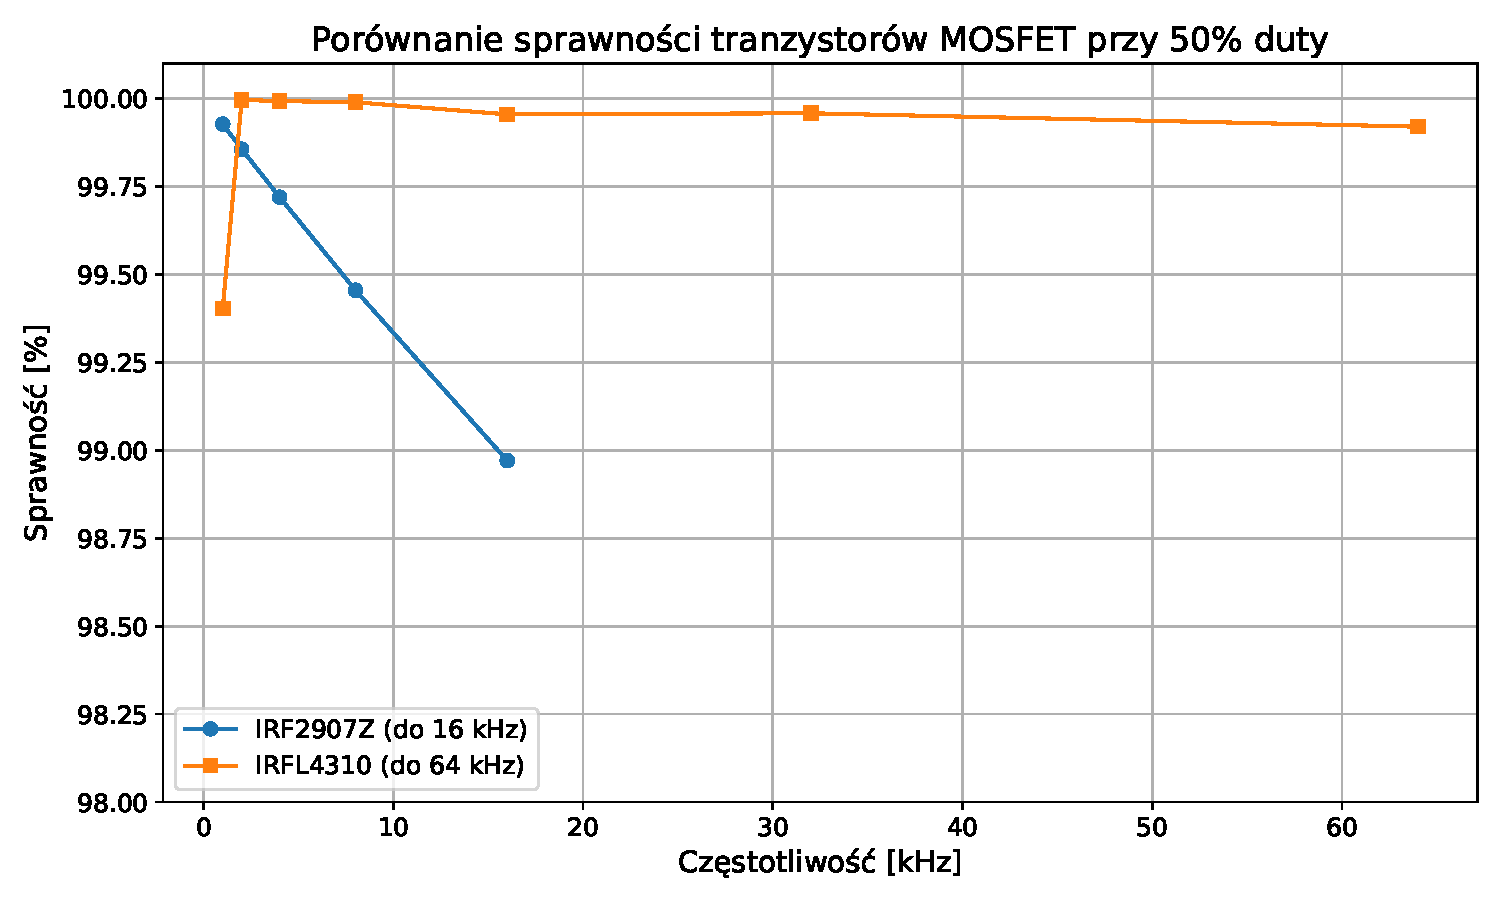
\includegraphics[width=0.8\textwidth]{aun1_imp_mosfet_comparison.pdf}
\caption{Wykres sprawności wzmacniaczy impulsowych MOSFET}
\end{figure}

Jak widzimy, tranzystor IRFL4310 o mniejszym ładunku bramki cechuje się większą sprawnością przy większych częstotliwościach (oraz jest w stanie w ogóle poprawnie przy nich pracować), natomiast tranzystor IRF2907Z
cechuje się większą sprawnosciia dla mniejszych częstotliwości, co czyni go lepszym wyborem dla zastosowań, gdzie
straty przewodzenia stanowią główny problem.\\

\subsection{ZJAWISKA W OBWODZIE D-S TRANZYSTORA WYNIKAJĄCE Z PARAMETRÓW PASOŻYTNICZYCH OBWODU}

d) Badanie wartości pasożytniczych w układzie RLD sterowanym tranzystorem MOSFET

\begin{figure}[H]
\centering
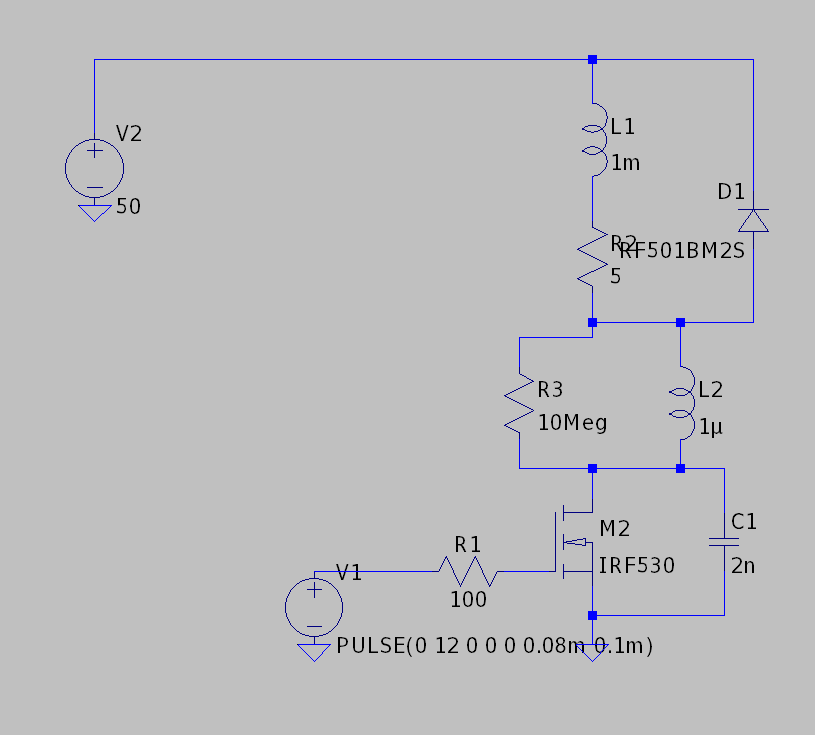
\includegraphics[width=0.8\textwidth]{aun1_rld_without_snubber.png}
\caption{Schemat pomiarowy układu RLD sterowanego tranzystorem MOSFET}
\end{figure}

\begin{figure}[H]
\centering
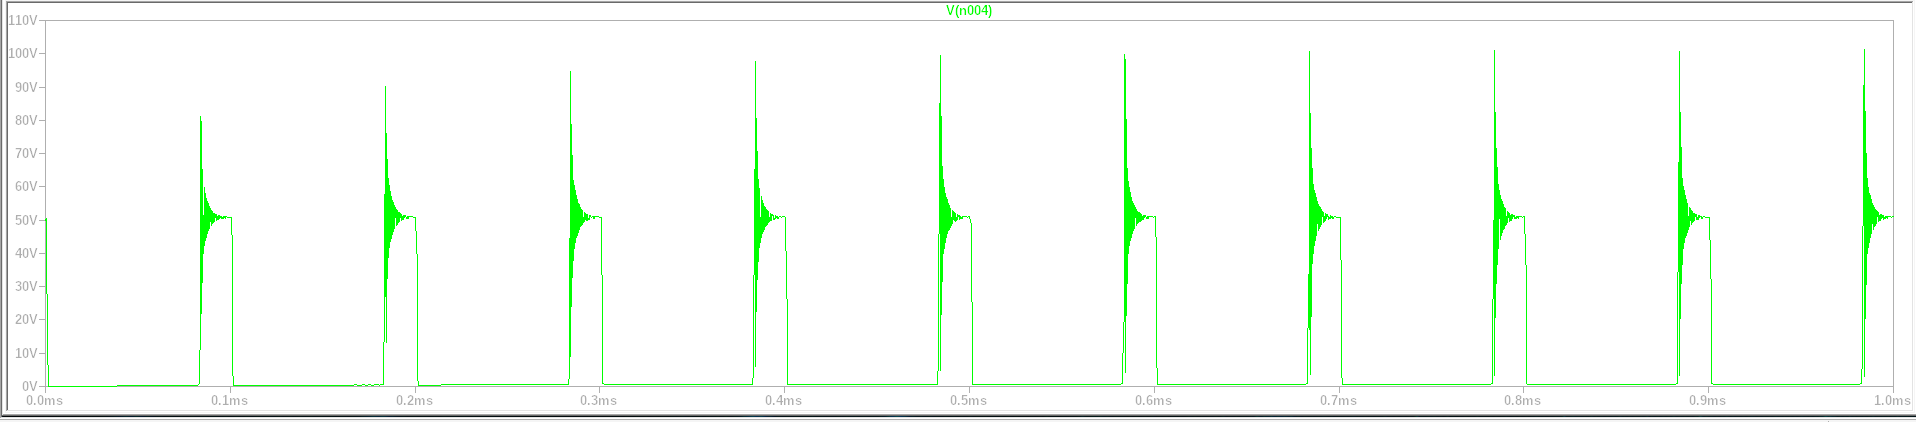
\includegraphics[width=0.8\textwidth]{aun1_rld_without_snubber_rgate100ohm.png}
\caption{Przebieg napięcia na wyjściu tranzystora MOSFET sterującego układem RLD z rezystancja bramki 100 [\Omega]}
\end{figure}

\begin{figure}[H]
\centering
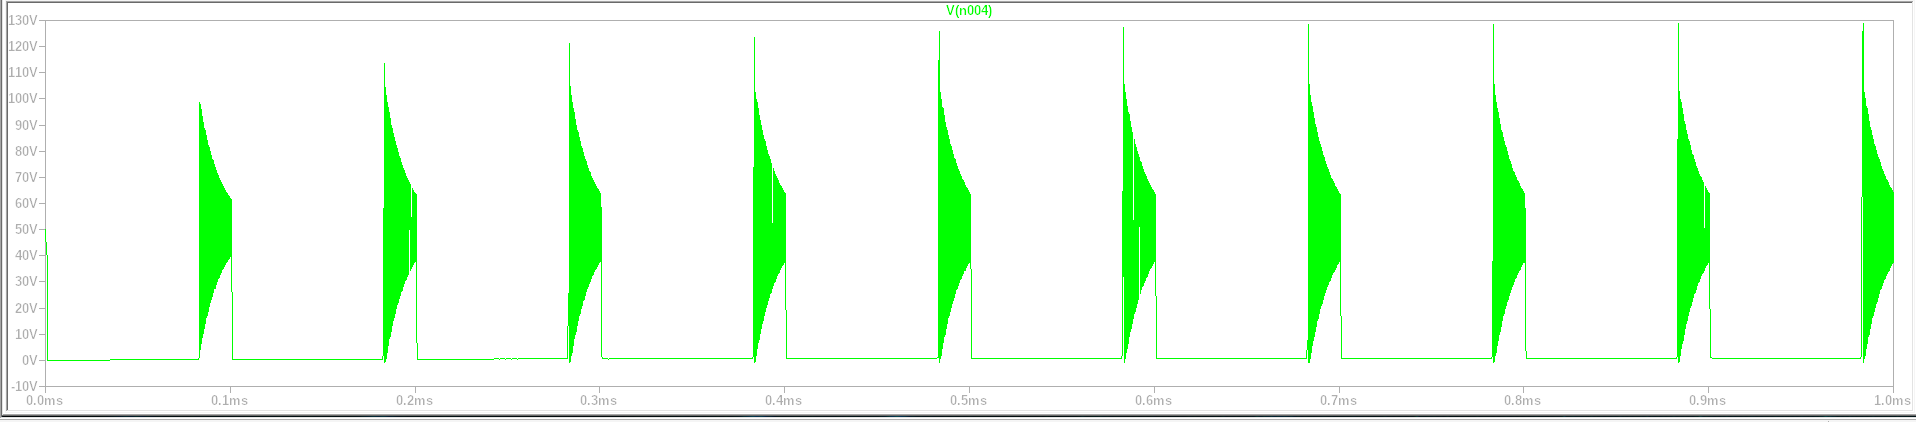
\includegraphics[width=0.8\textwidth]{aun1_rld_without_snubber_rgate10ohm.png}
\caption{Przebieg napięcia na wyjściu tranzystora MOSFET sterującego układem RLD z rezystancja bramki 10 [\Omega]}
\end{figure}

e) Dobór tłumika oscylacji napięcia (parametry snubber'a)

\begin{figure}[H]
\centering
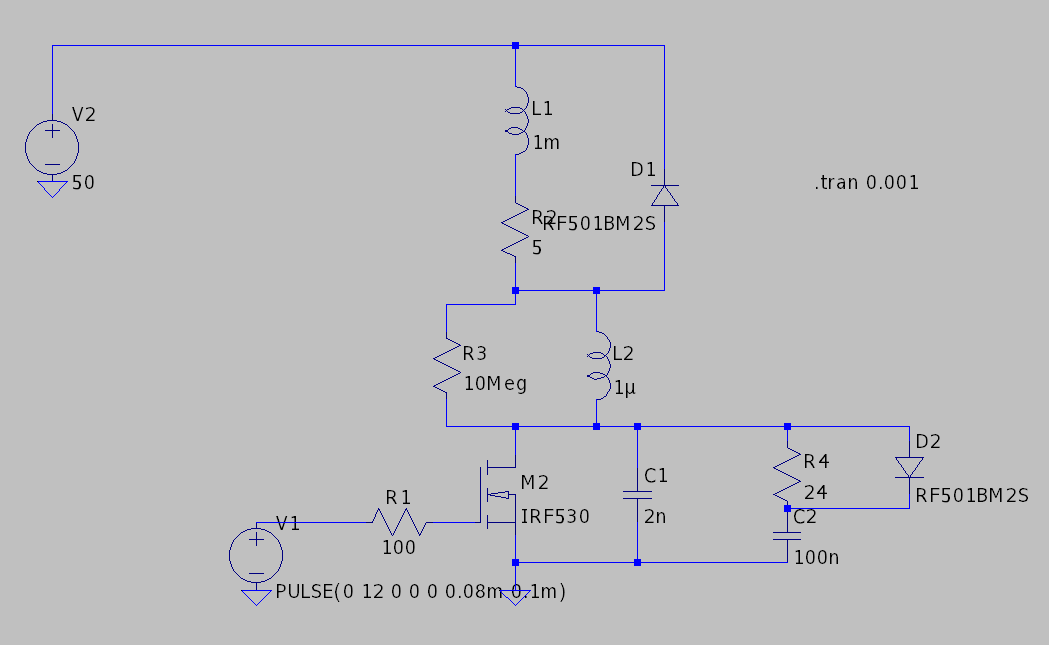
\includegraphics[width=0.8\textwidth]{aun1_rld_with_snubber.png}
\caption{Schemat pomiarowy układu RLD sterowanego tranzystorem MOSFET z tłumikiem oscylacji w obwodzie D-S tranzystora}
\end{figure}

Dobór parametrów tłumika (snubbera):
\begin{enumerate}
  \item Mierzymy częstotliwość oscylacji:
  \[
  f_0 = \SI{3.3}{\mega\hertz}
  \]
  \item Dobieramy kondensator o pojemności większej niż pojemność pasożytnicza tranzystora i mierzymy nową częstotliwość zakłóceń:
  \[
  C_1 = \SI{1}{\nano\farad}, \quad f_1 = \SI{2.7}{\mega\hertz}
  \]
  \item Liczymy stosunek częstotliwości:
  \[
  m = \frac{f_0}{f_1} = \frac{3.3}{2.7} = 1.22
  \]
  \item Obliczamy pojemność pasożytniczą tranzystora:
  \[
  C_0 = \frac{C_1}{m^2 - 1} = \frac{1\,\text{nF}}{1.22^2 - 1} = \SI{2.02}{\nano\farad}
  \]
  \item Obliczamy wartość indukcyjności pasożytniczej:
  \[
  L_0 = \frac{(m^2 - 1)}{(2\pi f_0)^2 C_1} = \frac{(1.22^2 - 1)}{(2\pi \cdot 3.3 \times 10^6)^2 \cdot 1 \times 10^{-9}} = \SI{1.15}{\micro\henry}
  \]
  \item Obliczamy minimalną wartość pojemności kondensatora snubbera:
  \[
  C_{\text{snubber}} = 3C_0 = 3 \cdot \SI{2.02}{\nano\farad} = \SI{6.06}{\nano\farad}
  \]
  \item Obliczamy wartość rezystancji w snubberze:
  \[
  R_{\text{snubber}} = \sqrt{\frac{L_0}{C_0}} = \sqrt{\frac{1.15 \times 10^{-6}}{2.02 \times 10^{-9}}} = \SI{24}{\ohm}
  \]
\end{enumerate}

\begin{figure}[H]
\centering
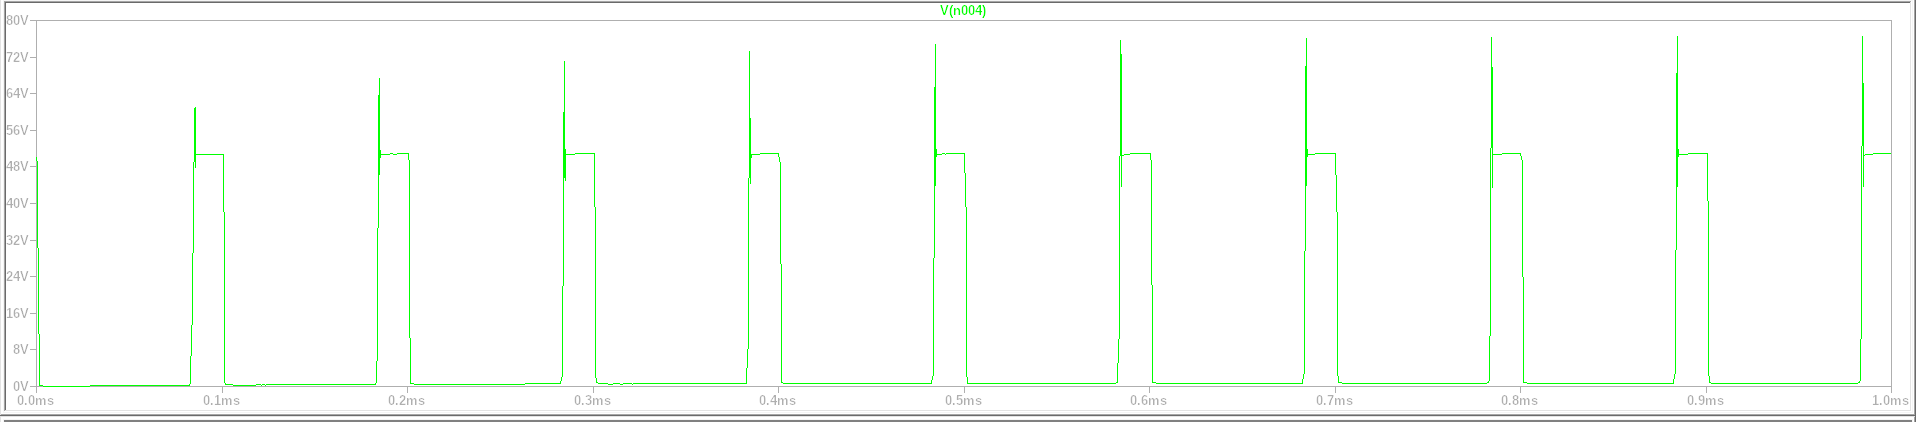
\includegraphics[width=0.8\textwidth]{aun1_rld_with_snubber_rgate100ohm.png}
\caption{Przebieg napięcia na wyjściu tranzystora MOSFET sterującego układem RLD z rezystancja bramki 100 [\Omega] i z tłumikiem oscylacji D-S}
\end{figure}

\begin{figure}[H]
\centering
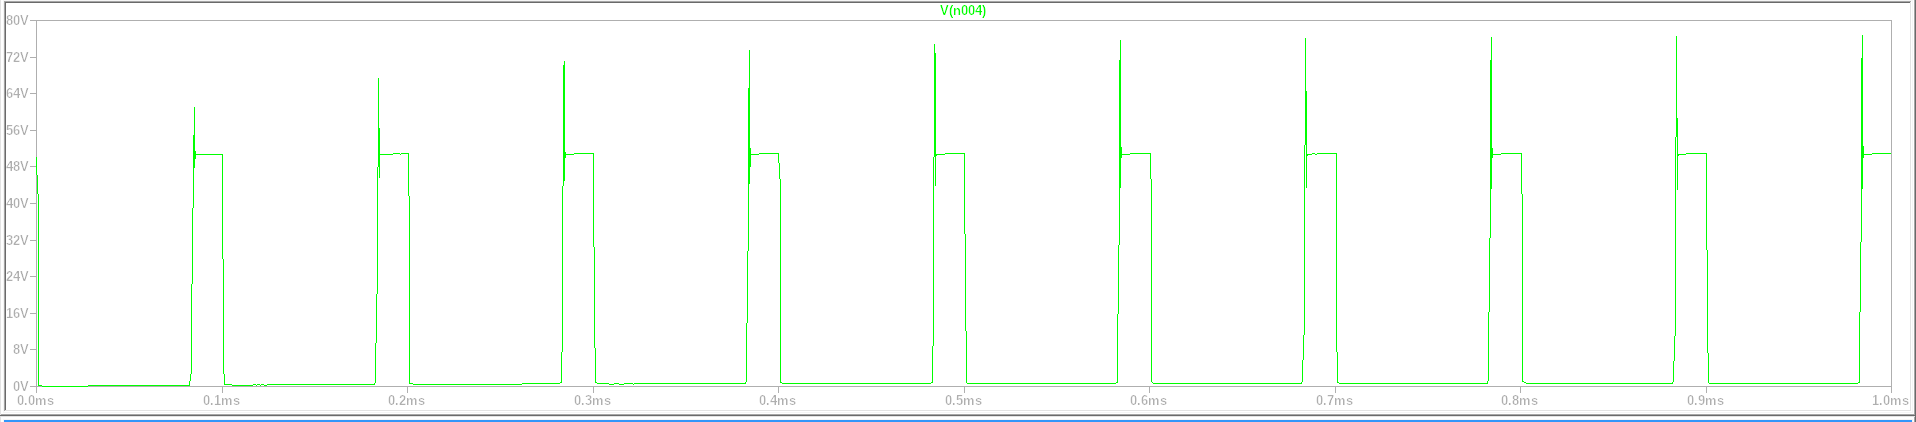
\includegraphics[width=0.8\textwidth]{aun1_rld_with_snubber_rgate10ohm.png}
\caption{Przebieg napięcia na wyjściu tranzystora MOSFET sterującego układem RLD z rezystancja bramki 10 [\Omega] i z tłumikiem oscylacji D-S}
\end{figure}

\begin{table}[H]
\centering
\begin{tabular}{|l|c|c|}
\hline
\textbf{Tłumik} & \(\mathbf{T_{ość} \ [\mu s]}\) & \(\mathbf{A_{ość} \ [V]}\) \\
\hline
Bez tłumika, \(R_{gate} = 100\,\Omega\) & 1.0958 & 30.7943 \\
\hline
Bez tłumika, \(R_{gate} = 10\,\Omega\) & 1.8058 & 50.8134 \\
\hline
Tłumik, \(R_{gate} = 10\,\Omega\) & 1.0968 & 10.0267 \\
\hline
Tłumik, \(R_{gate} = 100\,\Omega\) & 1.1505 & 10.4941 \\
\hline
\end{tabular}
\caption{Porównanie napięcia na drenie tranzystora MOSFET sterującym układem RLD z oraz bez użycia tłumika}
\label{tab:oscillation_data}
\end{table}

\end{figure}

\section{Część II}

\subsection{TYPOWA REALIZACJA TORU STEROWANIA TRANZYSTORA MOSFET}

f) Badanie wpływu wartości komponentów na stratę mocy na tranzystorze. Porównanie dynamiki transoptora analogowego i cyfrowego z uwzględnieniem prądu diody. Zależność wytracanej mocy na tranzystorze w zależności od częstotliwości PWM.

Zapoznano się ze strukturą i zamodelowano typowy tor sterowania tranzystorem MOSFET.
Układ składa się z bloku separacji galwanicznej – transoptora, układu wzmocnienia sygnału oraz gate drivera.
Transoptor zapewnia, że sygnał sterujący jest przekazywany bez elektrycznego połączenia, umożliwiając pracę w układzie o różnych punktach odniesienia masy i chroniąc elektronikę sterującą przed uszkodzeniem.
Gate driver odpowiada za szybkie i pewne przełączanie tranzystora poprzez odpowiednie ładowanie i rozładowywanie jego pojemności bramki, co ma istotny wpływ na straty przełączania oraz niezawodność pracy całego układu.
Do wejścia układu sterującego podawany jest sygnał PWM (ang. Pulse Width Modulation), który steruje pracą transoptora, a w konsekwencji – tranzystora MOSFET. Sygnał ten determinuje częstotliwość oraz czas włączenia tranzystora, wpływając bezpośrednio na charakterystykę napięcia i prądu w obwodzie wyjściowym.\\

\begin{figure}[H]
\centering
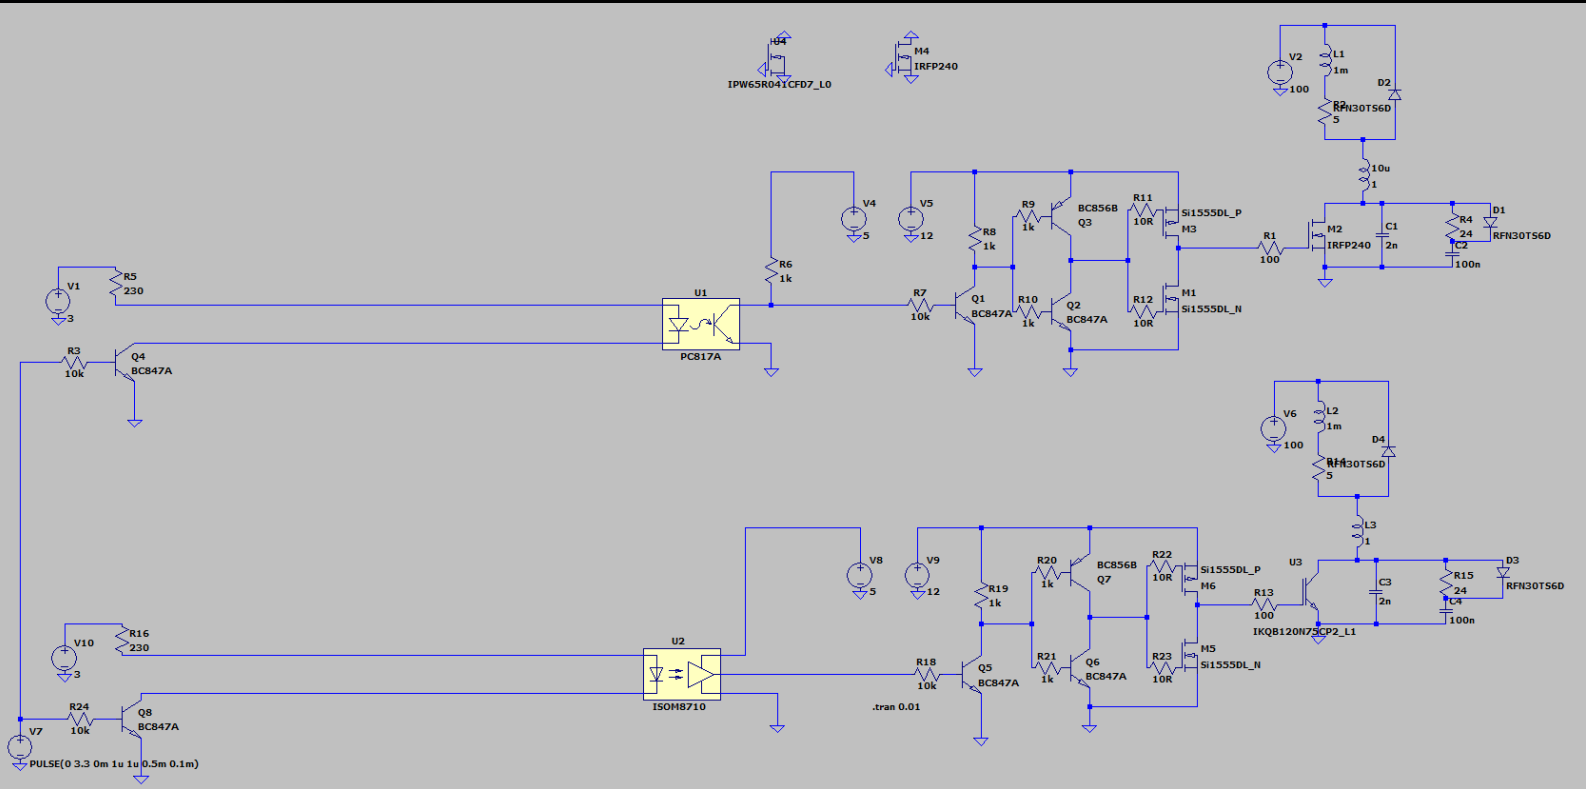
\includegraphics[width=0.8\textwidth]{aun1_transoptor.png}
\caption{Schemat pomiarowy toru sterowania tranzystora MOSFET}
\end{figure}

Porównano dwa transoptory - analogowy (PC817) oraz cyfrowy (ISOM8710). 
Dodatkowo zbadano wpływ prądu diody na ich dynamikę i przedstawiono na wykresach.\\

\begin{figure}[H]
\centering
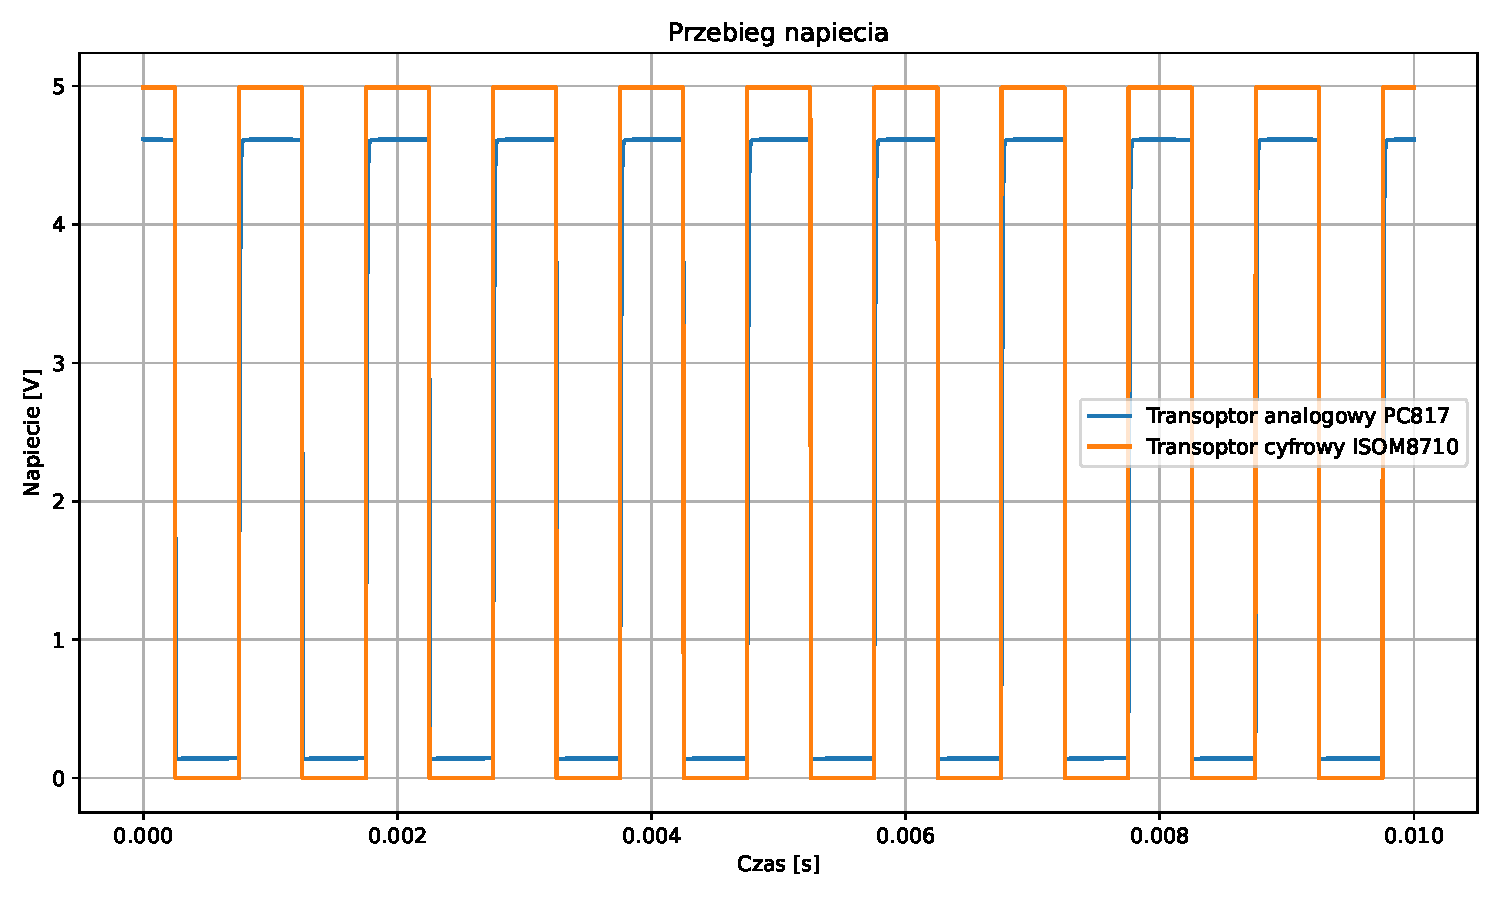
\includegraphics[width=0.8\textwidth]{aun1_gate_circuit_digital_vs_analog_rin100ohm.pdf}
\caption{Przebiegi napięcia na wyjściu tranzystora MOSFET z transoptorem dla rezystancji wejściowej 100 [\Omega]}
\end{figure}

\begin{figure}[H]
\centering
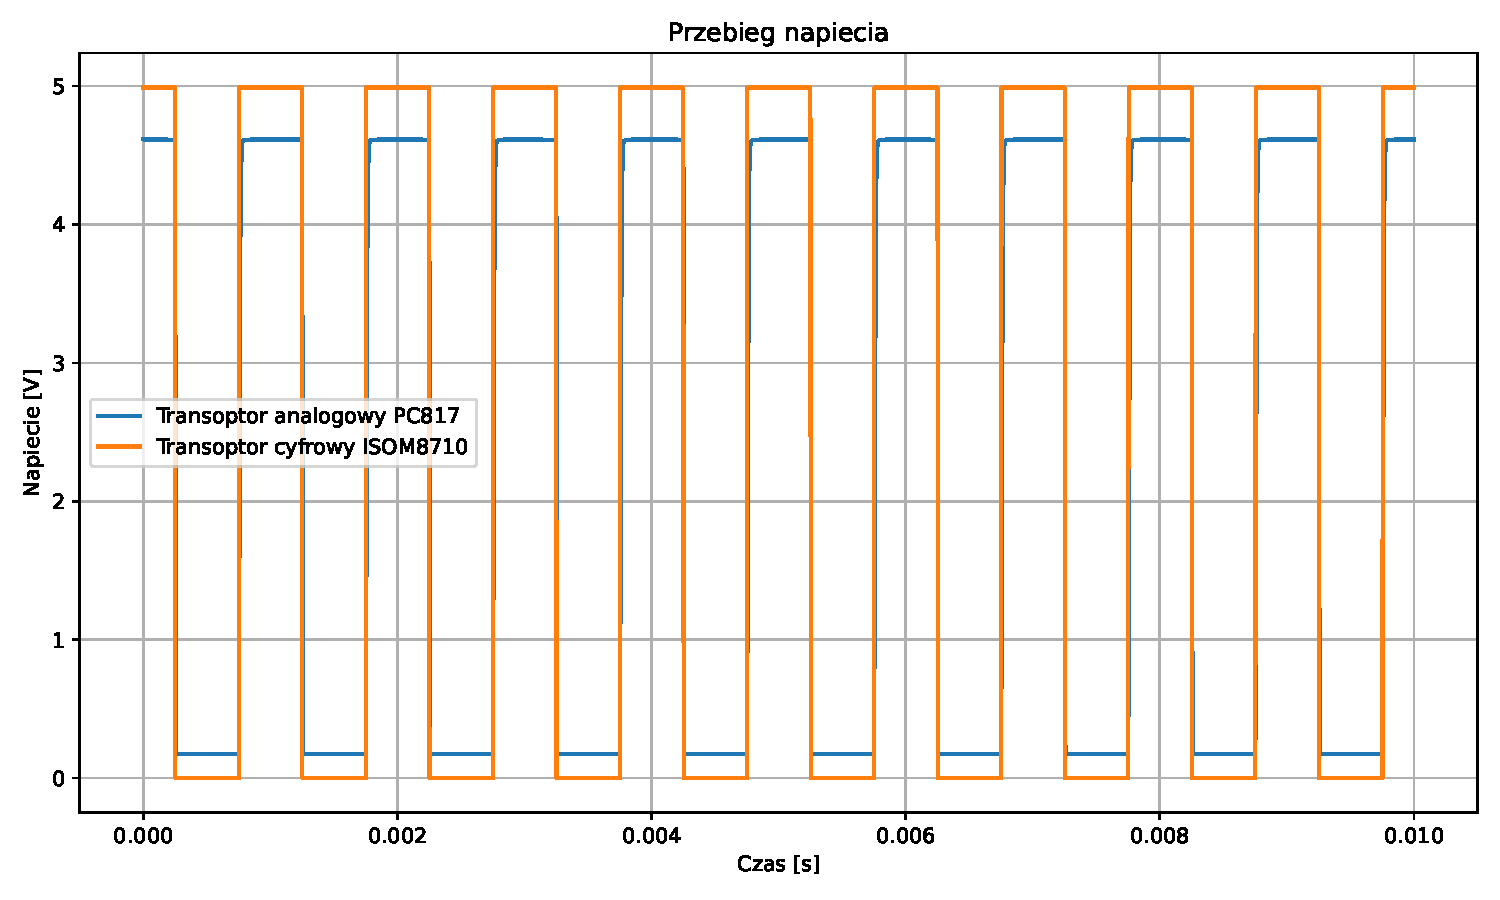
\includegraphics[width=0.8\textwidth]{aun1_gate_circuit_digital_vs_analog_rin230ohm.pdf}
\caption{Przebiegi napięcia na wyjściu tranzystora MOSFET z transoptorem dla rezystancji wejściowej 230 [\Omega]}
\end{figure}

\begin{figure}[H]
\centering
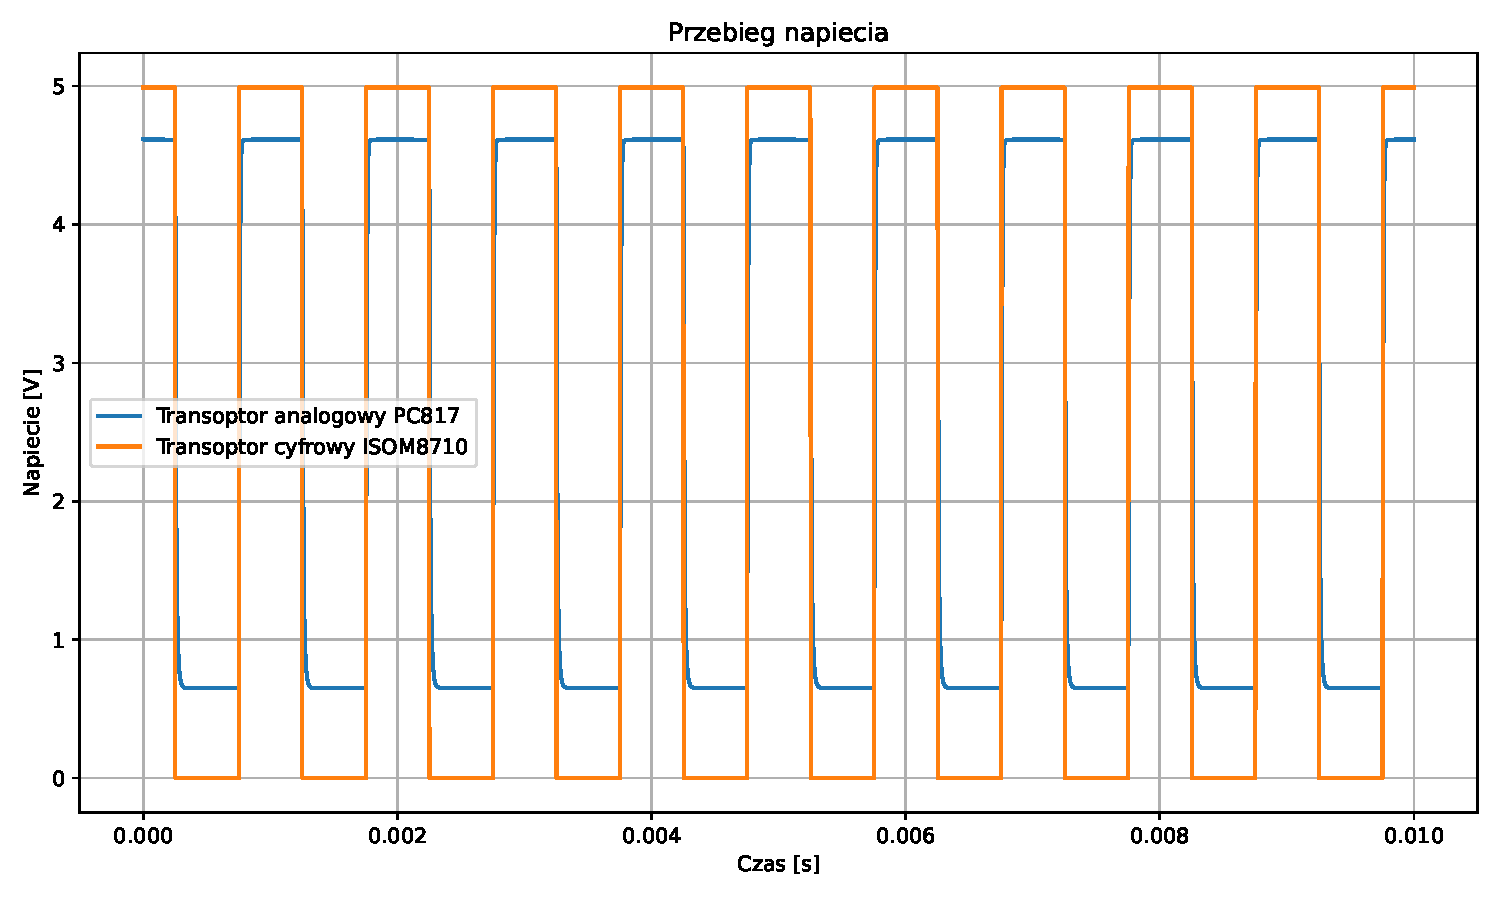
\includegraphics[width=0.8\textwidth]{aun1_gate_circuit_digital_vs_analog_rin500ohm.pdf}
\caption{Przebiegi napięcia na wyjściu tranzystora MOSFET z transoptorem dla rezystancji wejściowej 500 [\Omega]}
\end{figure}

\begin{figure}[H]
\centering
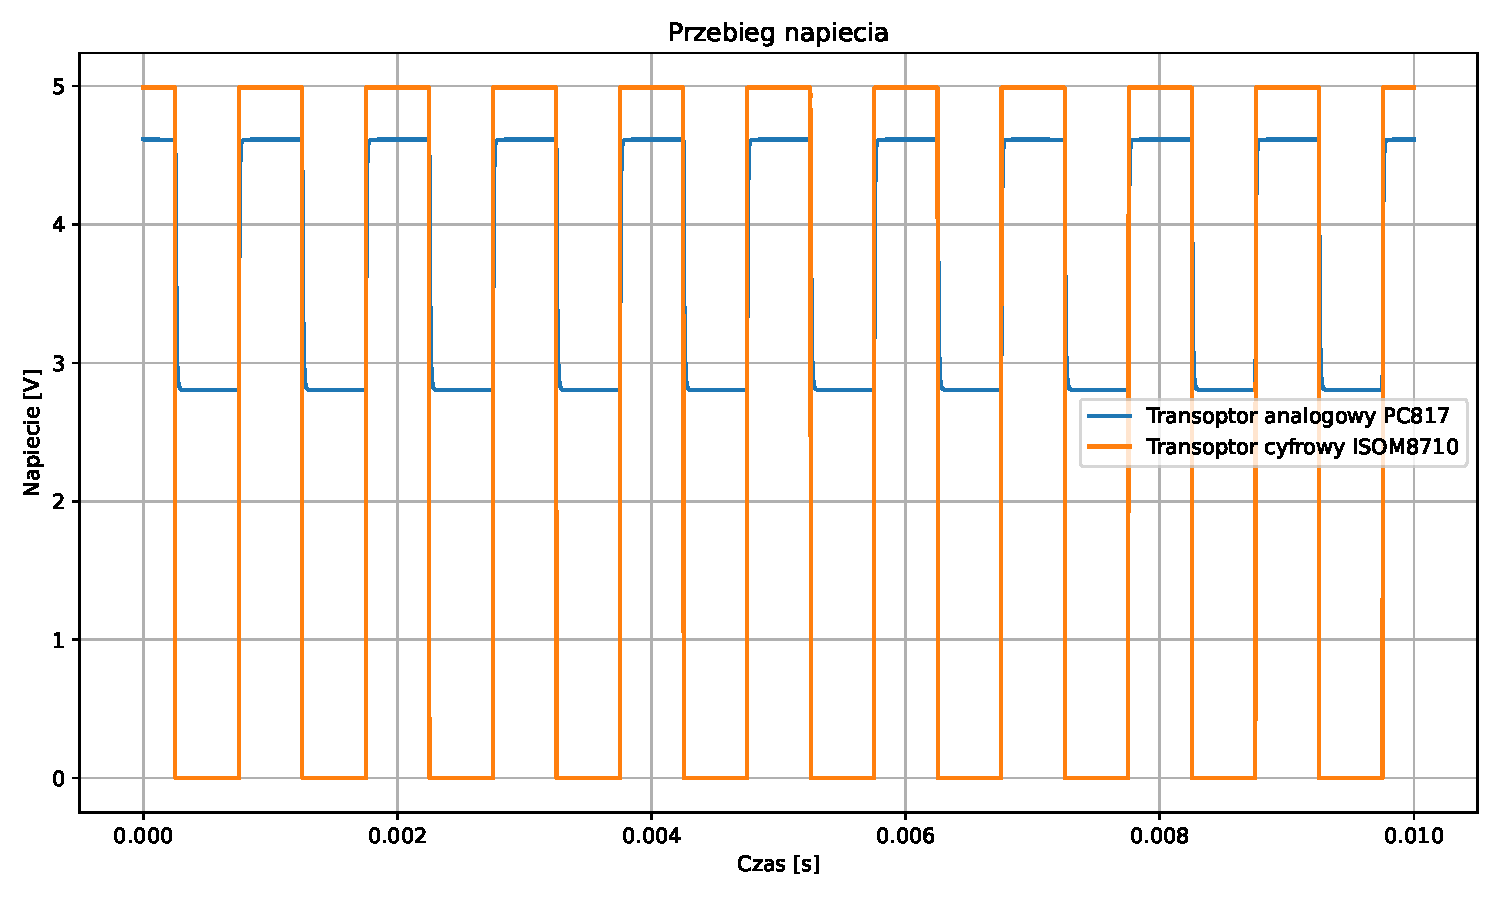
\includegraphics[width=0.8\textwidth]{aun1_gate_circuit_digital_vs_analog_rin1000ohm.pdf}
\caption{Przebiegi napięcia na wyjściu tranzystora MOSFET z transoptorem dla rezystancji wejściowej 1000 [\Omega]}
\end{figure}

\begin{table}[H]
\centering
\begin{tabular}{|l|c|c|}
\hline
\textbf{Rezystancja wejściowa} & \(\mathbf{I_{analog} \ [mA]}\) & \(\mathbf{I_{cyfrowy} \ [mA]}\) \\
\hline
100\,$\Omega$ & 18.0 & 14.0 \\
\hline
230\,$\Omega$ & 8.0 & 6.5 \\
\hline
500\,$\Omega$ & 3.8 & 3.2 \\
\hline
1000\,$\Omega$ & 1.9 & 1.6 \\
\hline
1560\,$\Omega$ & 1.3 & 1.0 \\
\hline
\end{tabular}
\caption{Porównanie prądu diody w funkcji rezystancji wejściowej dla sygnału analogowego i cyfrowego}
\label{tab:diode_current_comparison}
\end{table}

Z wykresów wynika, że im mniejszy prąd na diodzie, tym mniejsza minimalna wartość napięcia na transoptorze analogowym. Natomiast w przypadku transoptora cyfrowego napięcie minimalne nie ulega zmianie aż do momentu przekroczenia rezystancji $1560\ \Omega$ na rezystorze wejściowym — wtedy napięcie przyjmuje stałą wartość $5\ \mathrm{V}$.\\

Dynamika zmienia się także przy zmianie częstotliwości, co pokazano na wykresach: \\

\begin{figure}[H]
\centering
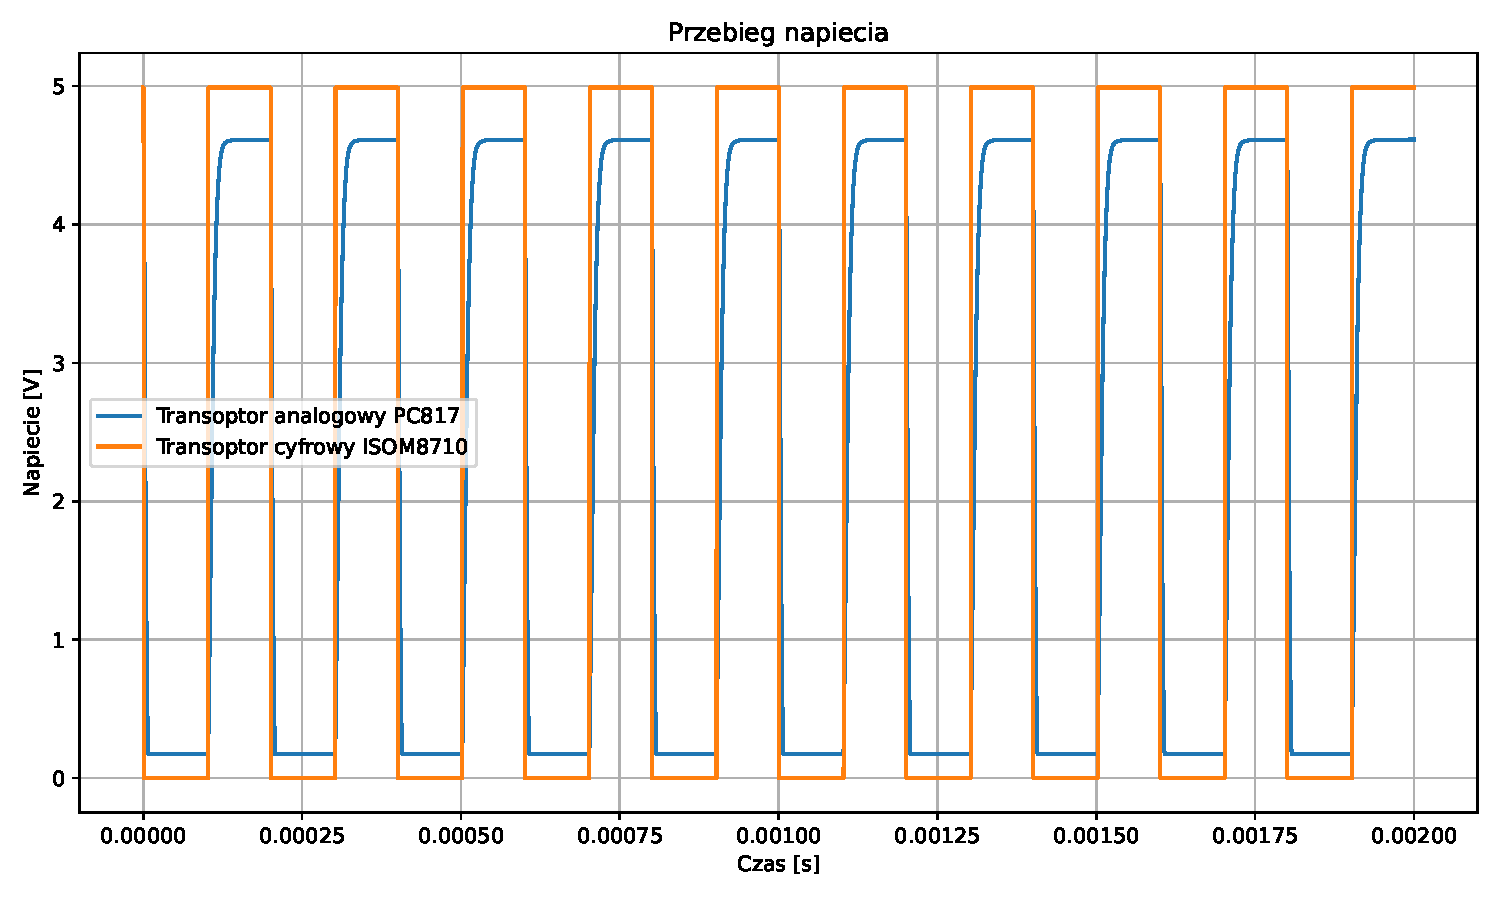
\includegraphics[width=0.8\textwidth]{aun1_gate_circuit_digital_vs_analog_5khz.pdf}
\caption{Przebiegi napięcia na wyjściu tranzystora MOSFET z transoptorem dla sygnału PWM o częstotliwości 5kHz}
\end{figure}

\begin{figure}[H]
\centering
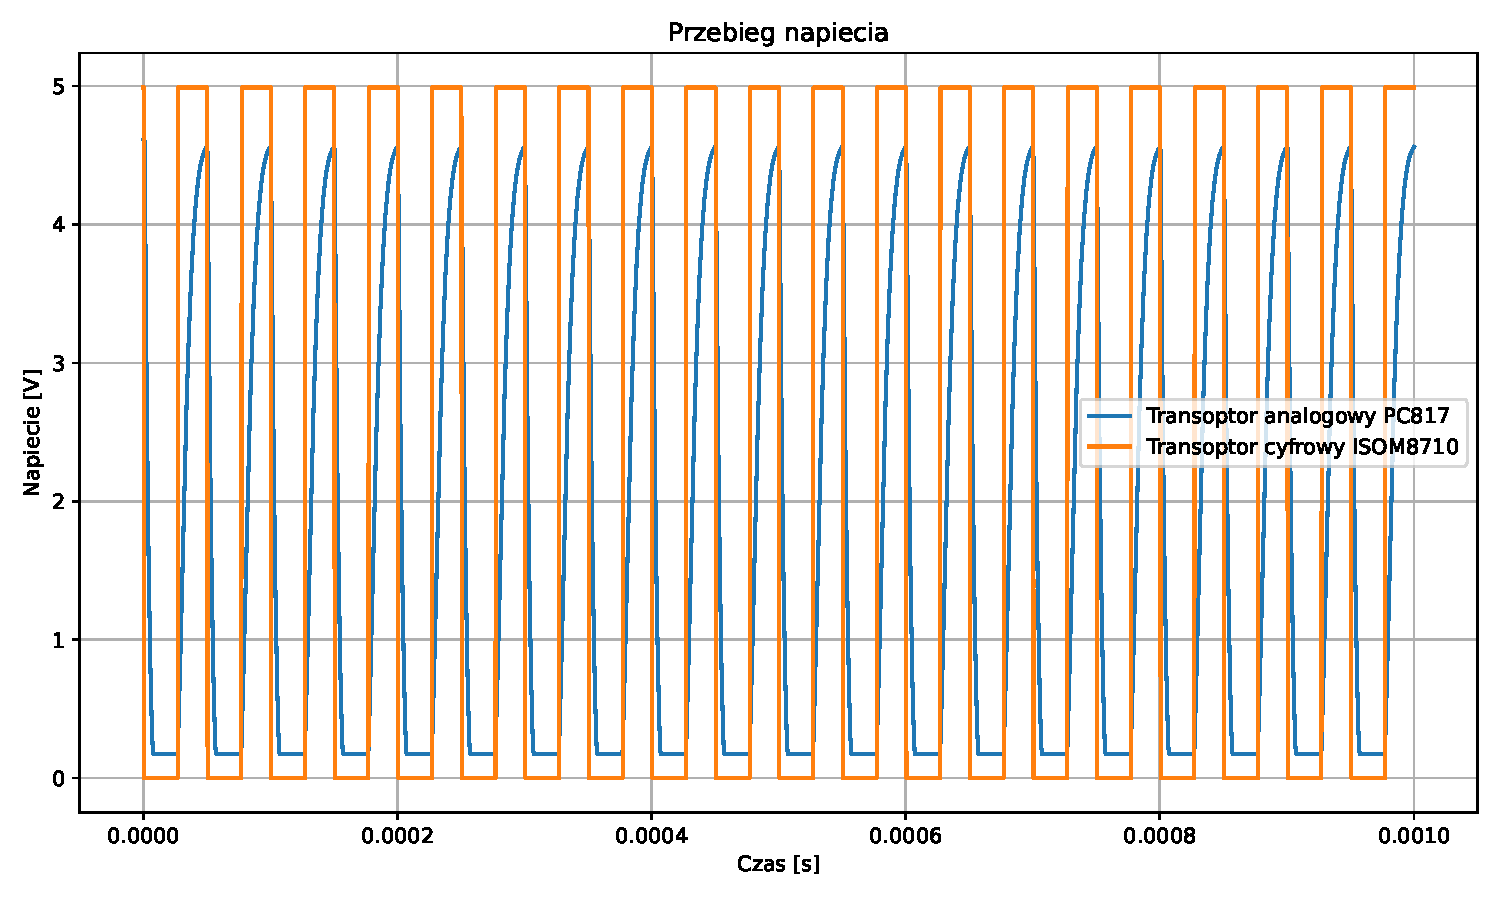
\includegraphics[width=0.8\textwidth]{aun1_gate_circuit_digital_vs_analog_20khz.pdf}
\caption{Przebiegi napięcia na wyjściu tranzystora MOSFET z transoptorem dla sygnału PWM o częstotliwości 20kHz}
\end{figure}

Na wykresach widać, że transoptor analogowy nie radzi sobie tak dobrze jak transoptor cyfrowy dla wysokich częstotliwości.\\

Zbadano średnią moc tranzystorów MOSFET IPW654041CFD7 (MOSFET) i IKQB120N75CP2 (IGBT). \\

\begin{table}[H]
\centering
\resizebox{\textwidth}{!}{%
\begin{tabular}{|l|c|c|}
\hline
\textbf{Częstotliwość [kHz]} & \textbf{Moc wytrącana IPW65R041CFD7 (W)} & \textbf{Moc wytrącana IKQB120N75CP2 (W)} \\
\hline
1 & 3.5 & 6.6 \\
\hline
5 & 2.2 & 6.4 \\
\hline
10 & 2.5 & 8.33 \\
\hline
25 & 3.8 & 14.8 \\
\hline
50 & 6.1 & 26.8 \\
\hline
100 & 12.1 & 52.3 \\
\hline
\end{tabular}%
}
\caption{Średnia moc wytrącaną na tranzystorze w zależności od częstotliwości}
\end{table}

Widać, że im większa częstotliwość tym większe straty na tranzystorach. Patrząc na straty mocy to lepiej radzi sobie tranzystor IPW654041CFD7, niż IKQB120N75CP2.\\

\subsection{MOSTKOWE UKŁADY WZMACZNIACZY TRANZYSTOROWYCH}

g) Problemy mostków mocy

Mostek mocy to układ elektroniczny wykorzystywany do sterowania przepływem prądu przez obciążenie, najczęściej silnik. Najpopularniejszą konfiguracją jest tzw. mostek H, który składa się z czterech tranzystorów mocy. Dzięki odpowiedniemu przełączaniu tych tranzystorów możliwe jest sterowanie kierunkiem oraz wartością prądu płynącego przez obciążenie. Mostki mocy znajdują zastosowanie w układach napędowych i przekształtnikach, a ich działanie opiera się na szybkim przełączaniu elementów półprzewodnikowych w celu efektywnego zarządzania energią.\\

W mostku H kluczowe są trzy rodzaje sterowania:
\begin{itemize}
\item unipolarny,
\item quasi-bipolarny,
\item bipolarny.
\end{itemize}
\vspace{1em}

h) Analiza działania układu sterowania bipolarnego, unipolarnego, quasi-bipolarnego

W układach z obciążeniem RLE (rezystancja, indukcyjność i źródło siły elektromotorycznej), istotnym zjawiskiem jest konieczność zapewnienia ścieżki demagnetyzacji dla prądu cewki. Podczas wyłączania tranzystorów sterujących, energia zgromadzona w indukcyjności nie może zostać natychmiast rozproszona. W takim przypadku pojawiają się przepięcia i zakłócenia, o ile nie zostanie zapewniona odpowiednią ścieżka dla tego prądu.\\

\textbf{Sterowanie unipolarne:}
W tym trybie tranzystory włączane są na przemian tylko w jednej gałęzi mostka (np. górnej). Prąd powrotny z cewki płynie przez diody swobodne w dolnej gałęzi. Ścieżka demagnetyzacji realizowana jest wyłącznie przez te diody, co powoduje wolniejszą dynamikę wyłączania i dłuższy czas ustalania się prądu.
Napięcie wyjściowe przyjmuje wartości +U oraz 0 V, ponieważ prąd jest kierowany tylko przez jedną gałąź mostka, a powrót odbywa się przez diody swobodne.\\

\textbf{Sterowanie quasi-bipolarne:}
Jest to tryb pośredni, gdzie w każdej połowie okresu włączany jest jeden tranzystor, natomiast przeciwny tranzystor w drugiej gałęzi jest wyłączony. Demagnetyzacją cewki odbywa się przez diody swobodne przeciwległej gałęzi, które stanowią naturalną ścieżkę dla prądu indukowanego. Dzięki temu dynamika pracy jest lepszą niż w trybie unipolarnym, a układ zachowuje prostotę sterowania i mniejsze straty energetyczne.
Napięcie może przyjmować wartości +U, –U oraz 0 V, ponieważ każda z połówek cyklu wykorzystuje inną gałąź mostka. Zmiana polaryzacji odbywa się za pośrednictwem diod swobodnych, co umożliwia krótkotrwałe stany zerowe.\\

\textbf{Sterowanie bipolarne:}
Tranzystory włączane są naprzemiennie w obu gałęziach mostka, co pozwala na aktywne sterowanie przepływem prądu w obydwu kierunkach. W momencie przełączania prąd z cewki jest wymuszany przez aktywnie sterowany tranzystor w drugiej gałęzi, co zapewnia najszybszą i najbardziej precyzyjną ścieżkę demagnetyzacji. Odbywa się to jednak kosztem wyższych strat mocy i bardziej skomplikowanego układu sterowania.
Napięcie wyjściowe skacze bezpośrednio między +U a –U. W idealnym przypadku nie występuje 0 V, chyba że w czasie przełączeń PWM (np. dead-time). Umożliwia to najbardziej dynamiczne sterowanie prądem.\\

\begin{figure}[H]
\centering
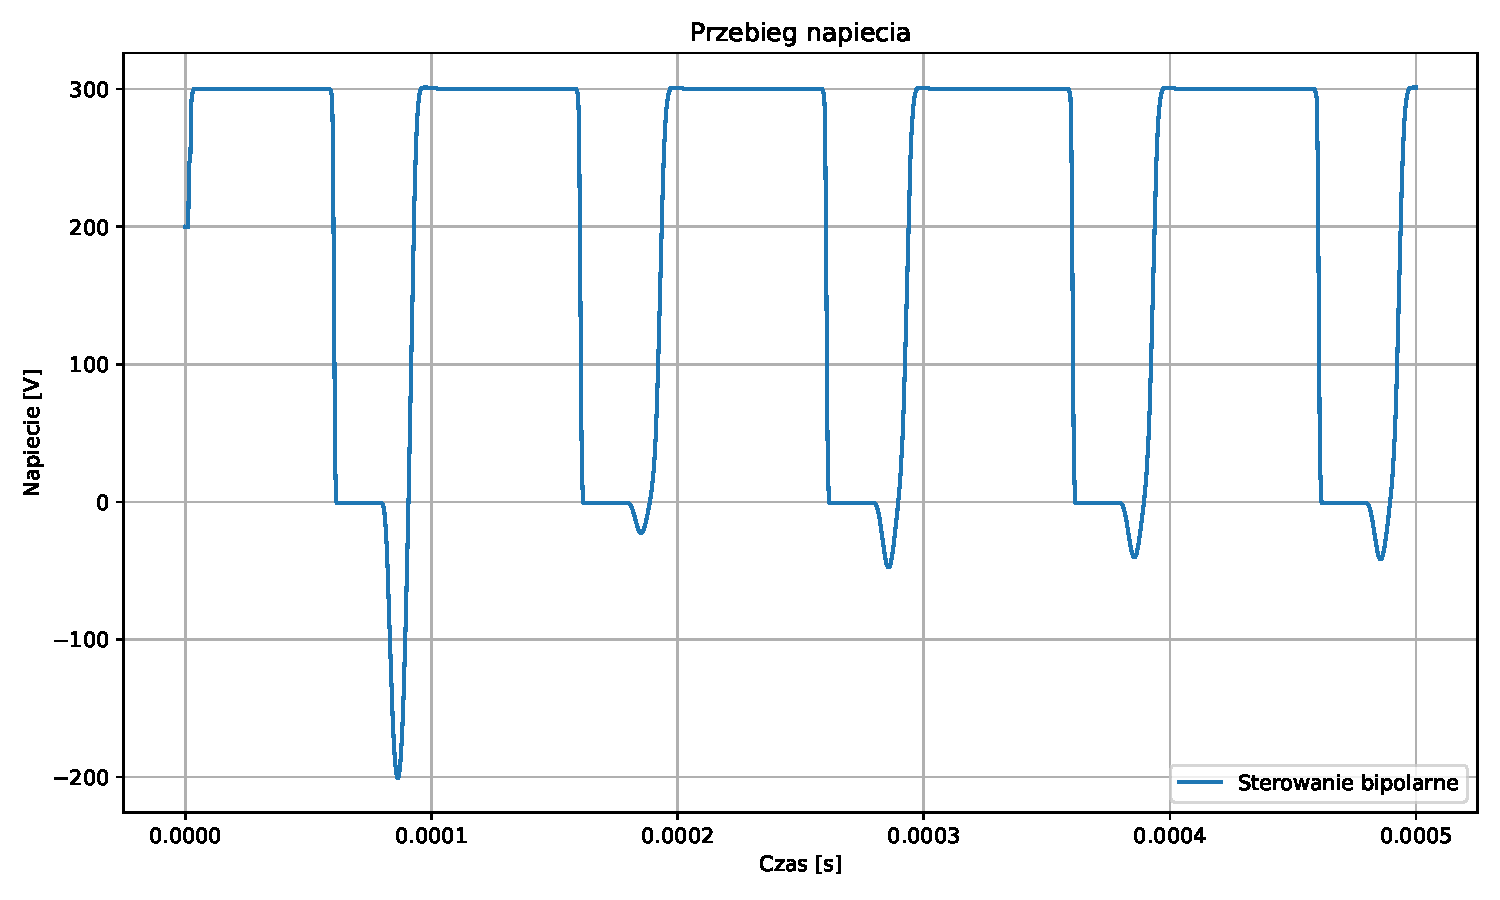
\includegraphics[width=0.8\textwidth]{aun1_bipolar_motor.pdf}
\caption{Przebieg napięcia na silniku przy mostku sterowanym bipolarnie}
\end{figure}

\begin{figure}[H]
\centering
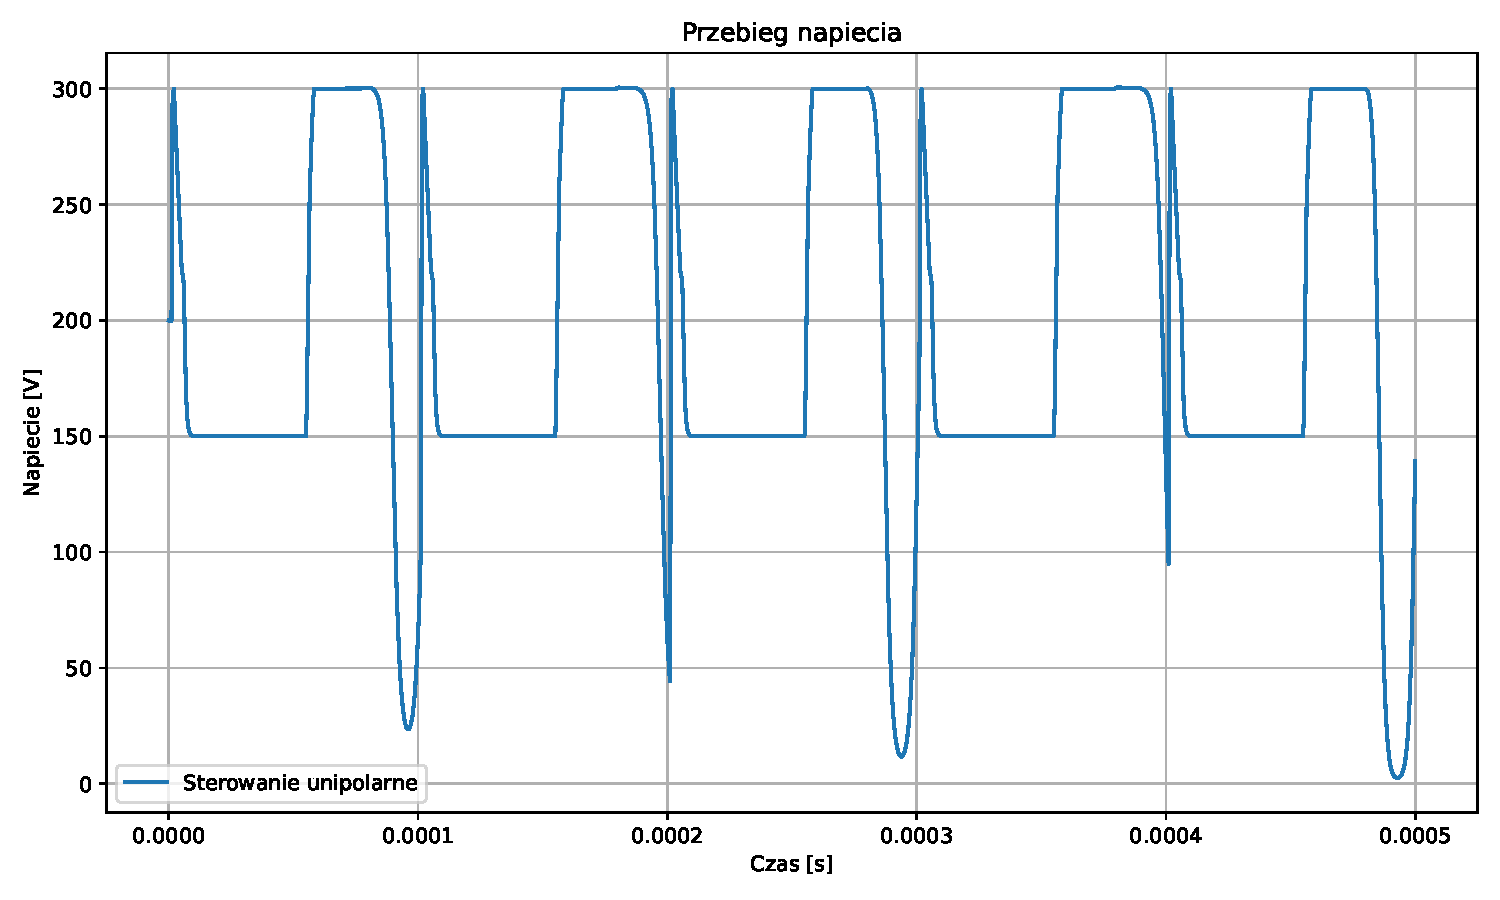
\includegraphics[width=0.8\textwidth]{aun1_unipolar_motor.pdf}
\caption{Przebieg napięcia na silniku przy mostku sterowanym unipolarnie}
\end{figure}

i) Model bipolarnego i unipolarnego sterowania

Zamodelowano w matlabie i pokazano na wykresach sterowanie bipolarne i unipolarne silnika oraz jak to wpływa na jego prędkość:\\

\begin{figure}[H]
\centering
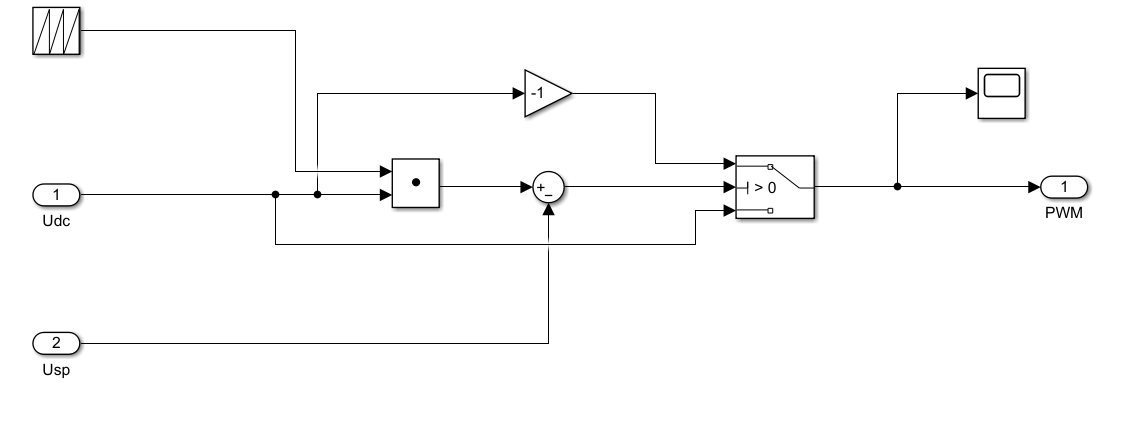
\includegraphics[width=0.8\textwidth]{aun1_bipolar_schematic.png}
\caption{Schemat pomiarowy mostka sterowanego bipolarnie}
\end{figure}

\begin{figure}[H]
\centering
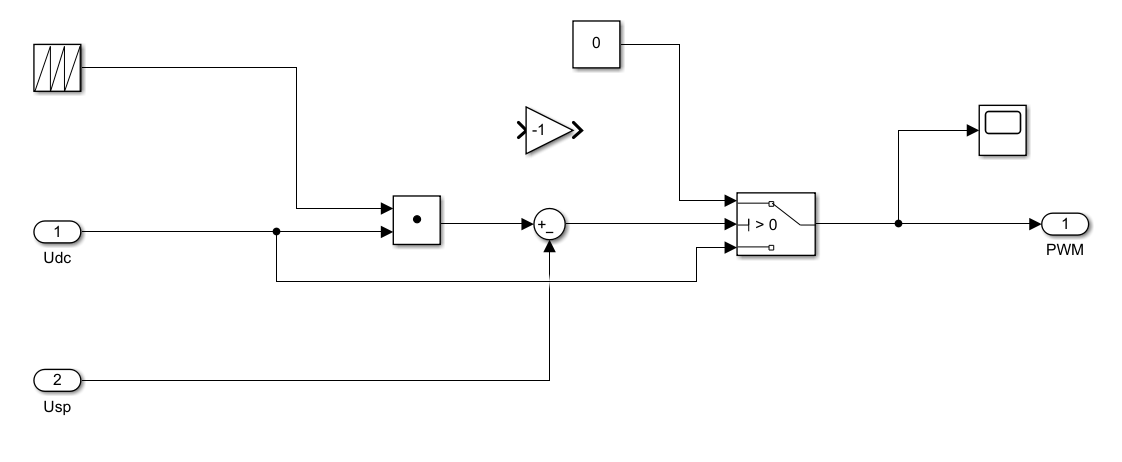
\includegraphics[width=0.8\textwidth]{aun1_unipolar_schematic.png}
\caption{Schemat pomiarowy mostka sterowanego unipolarnie}
\end{figure}

\begin{figure}[H]
\centering
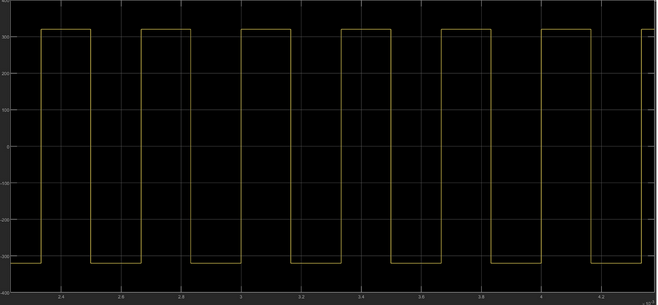
\includegraphics[width=0.8\textwidth]{aun1_bipolar_bridge_voltage.png}
\caption{Przebieg napięcia na silniku przy mostku sterowanym bipolarnie}
\end{figure}

\begin{figure}[H]
\centering
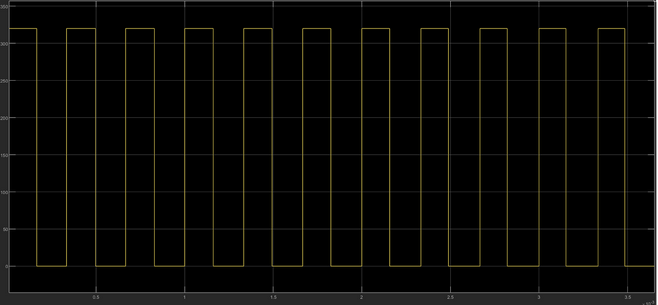
\includegraphics[width=0.8\textwidth]{aun1_unipolar_bridge_voltage.png}
\caption{Przebieg napięcia na silniku przy mostku sterowanym unipolarnie}
\end{figure}

\begin{figure}[H]
\centering
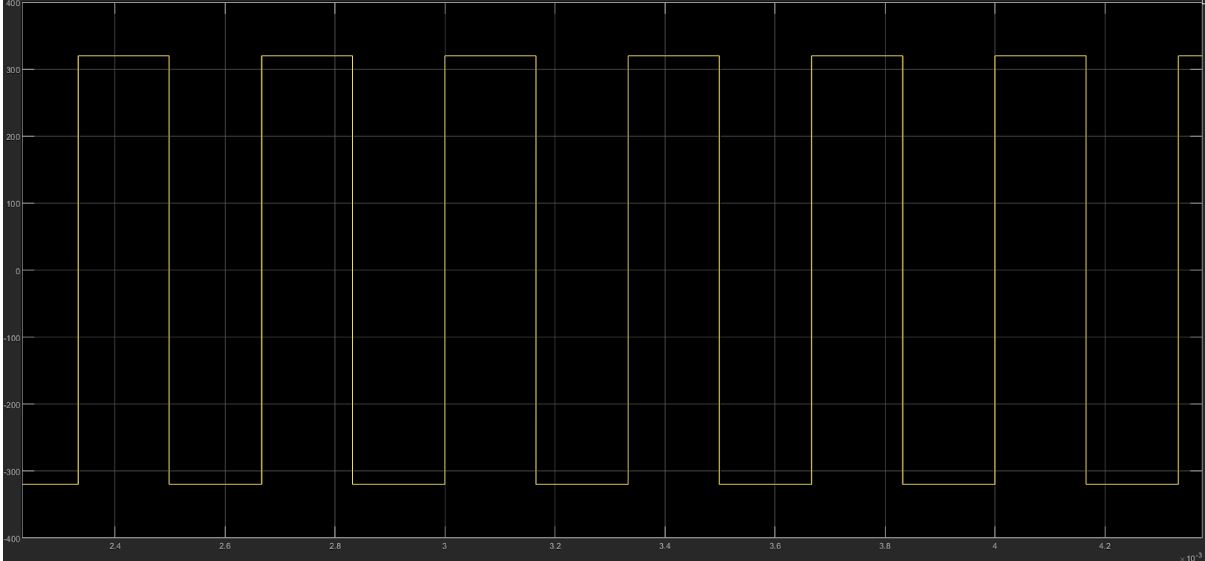
\includegraphics[width=0.8\textwidth]{aun1_bipolar_bridge.png}
\caption{Przebieg prędkości na silniku przy mostku sterowanym bipolarnie}
\end{figure}

\begin{figure}[H]
\centering
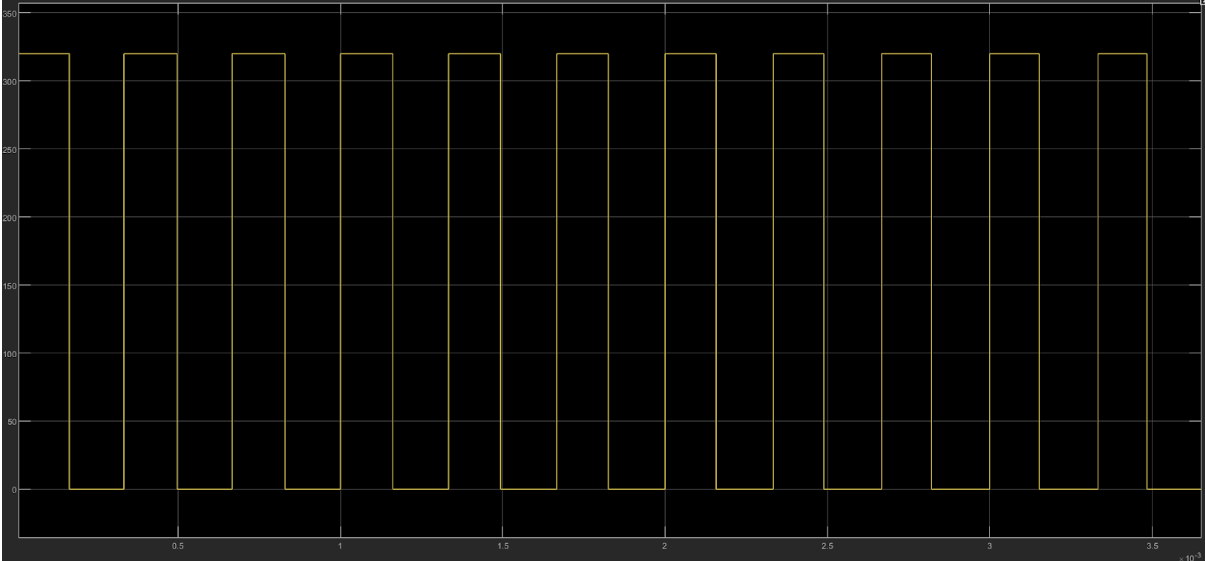
\includegraphics[width=0.8\textwidth]{aun1_unipolar_bridge.png}
\caption{Przebieg prędkości na silniku przy mostku sterowanym unipolarnie}
\end{figure}

Z wykresów wynika, że przy sterowaniu unipolarnym dynamika układu jest gorsza, a odpowiedź ustala się wolniej. Sterowanie to jest jednak bardziej efektywne energetycznie.\\

\section{Część III}

\subsection{BADANIA EKSPERYMENTALNE}

j) Przebiegi prądów oraz napięć na stanowiskach eksperymentalnych

Uwaga: brak jednostek na osi OY spowodowany jest faktem, że dane
zapisane były w formacie raw, niezeskalowane.\\

Regulacja prędkości odbywa się przez zmianę częstotliwości prądu i napięcia, amplituda pozostaje stała.\\

Przebiegi napięcia i prądu na stanowisku Alspa.\\

\begin{figure}[H]
\centering
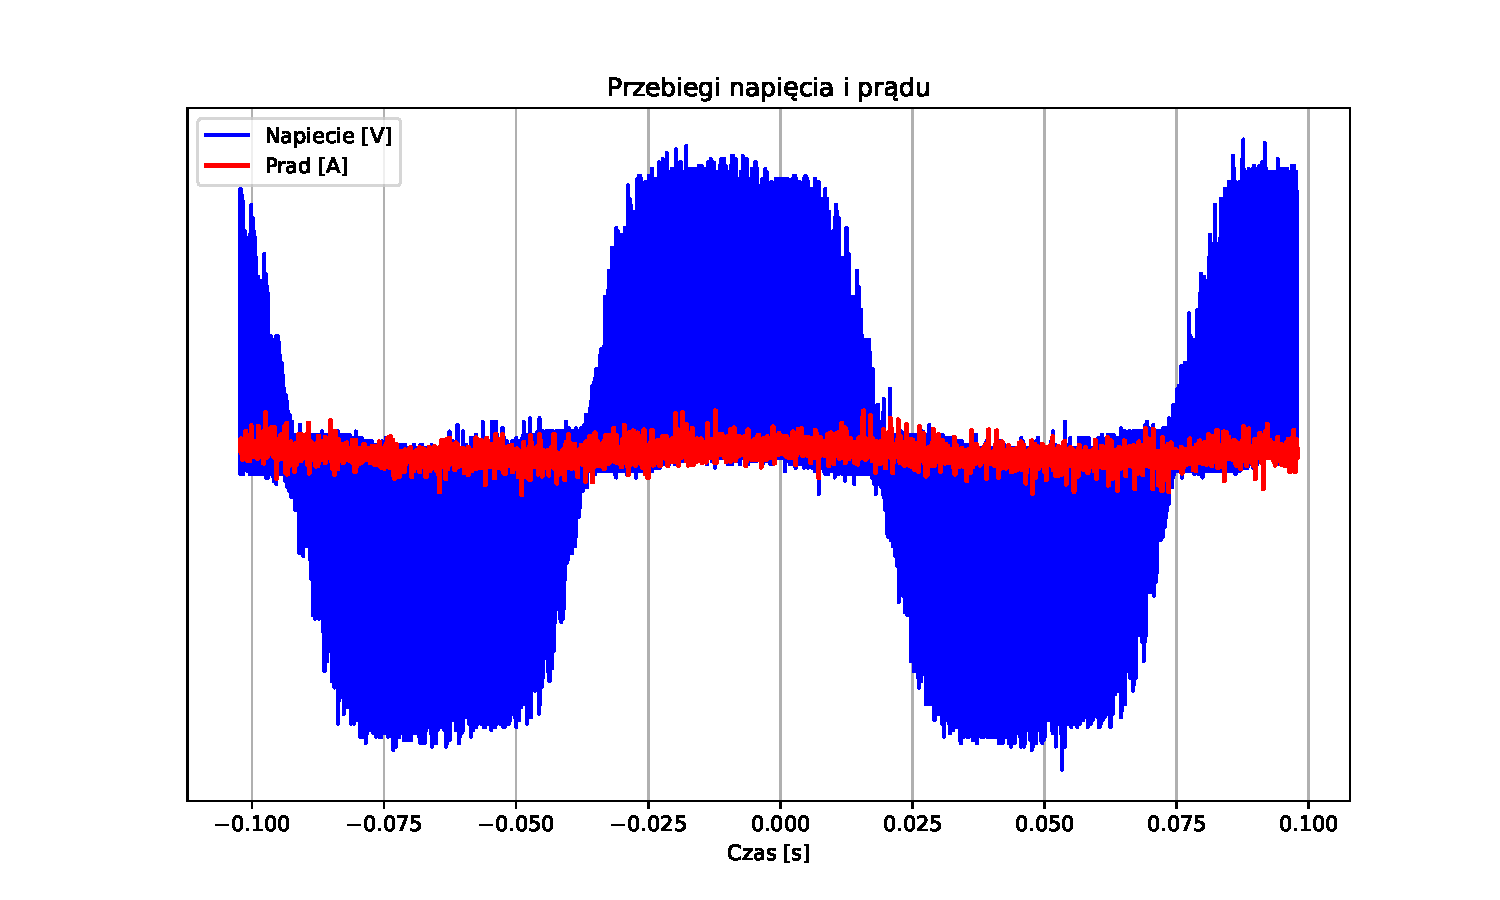
\includegraphics[width=0.8\textwidth]{aun1_alspa_rpm300.pdf}
\caption{Przebieg napięcia oraz prądu na stanowisku Alspa przy prędkości kątowej 300 [RPM]}
\end{figure}

\begin{figure}[H]
\centering
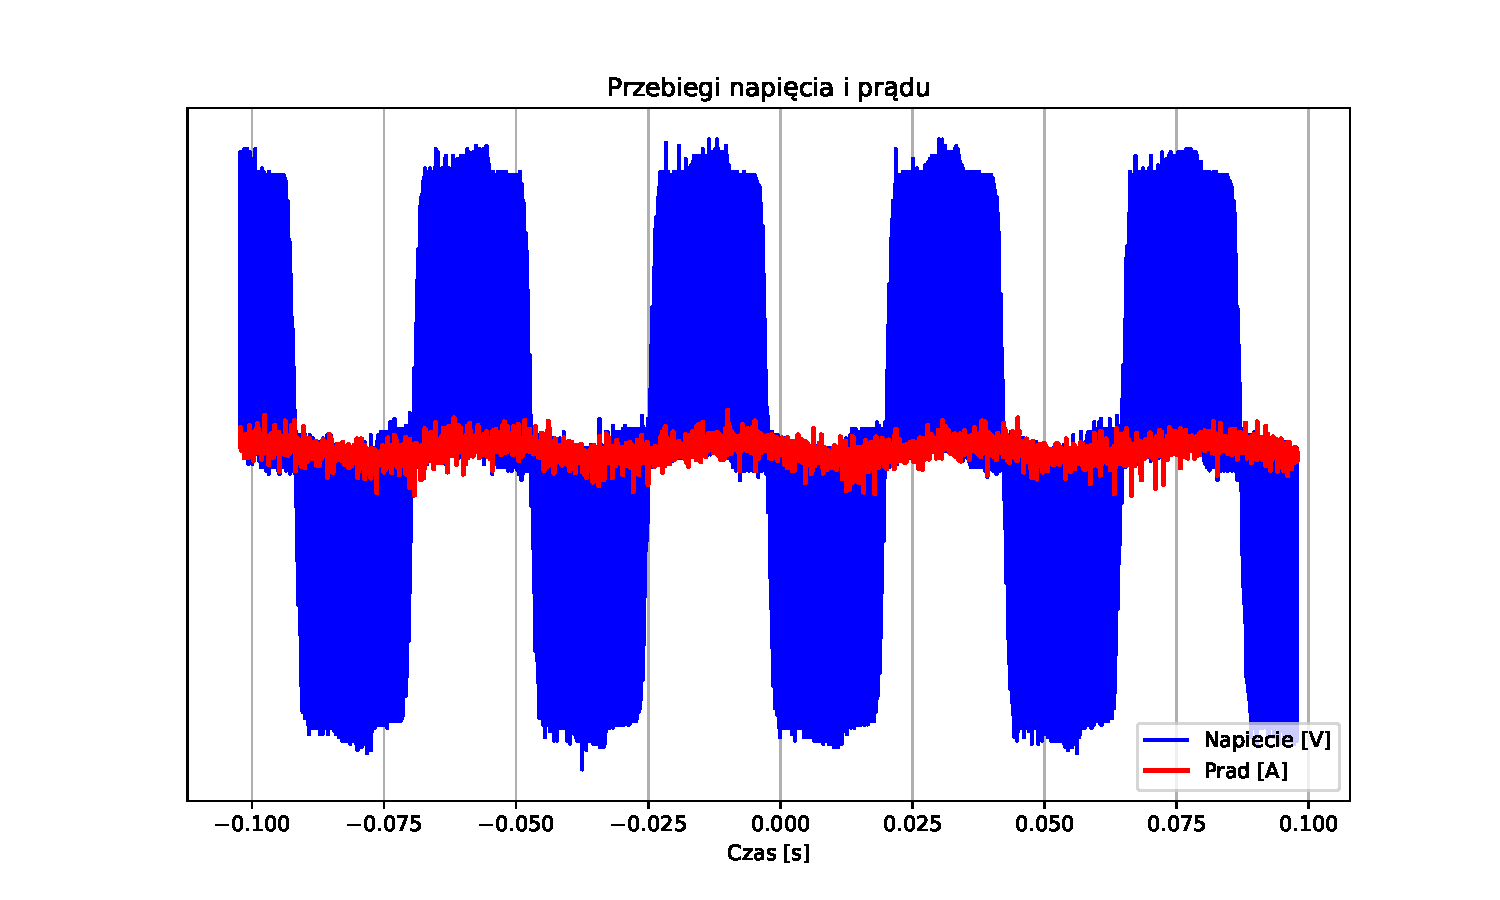
\includegraphics[width=0.8\textwidth]{aun1_alspa_rpm600.pdf}
\caption{Przebieg napięcia oraz prądu na stanowisku Alspa przy prędkości kątowej 600 [RPM]}
\end{figure}

\begin{figure}[H]
\centering
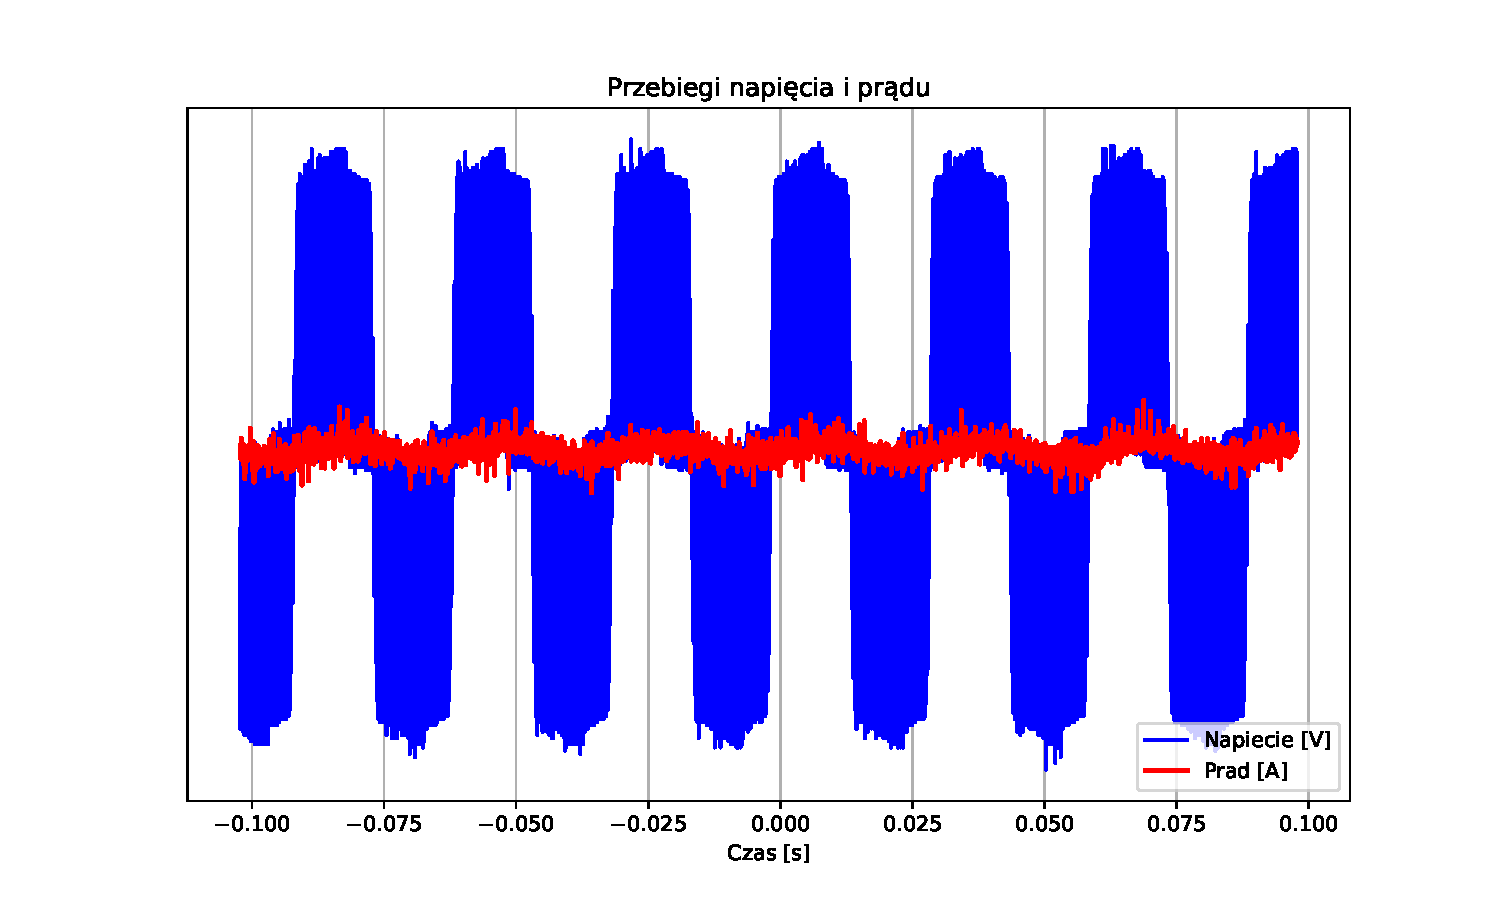
\includegraphics[width=0.8\textwidth]{aun1_alspa_rpm900.pdf}
\caption{Przebieg napięcia oraz prądu na stanowisku Alspa przy prędkości kątowej 900 [RPM]}
\end{figure}

Przebiegi napięcia i prądu na stanowisku Microverter.\\

\begin{figure}[H]
\centering
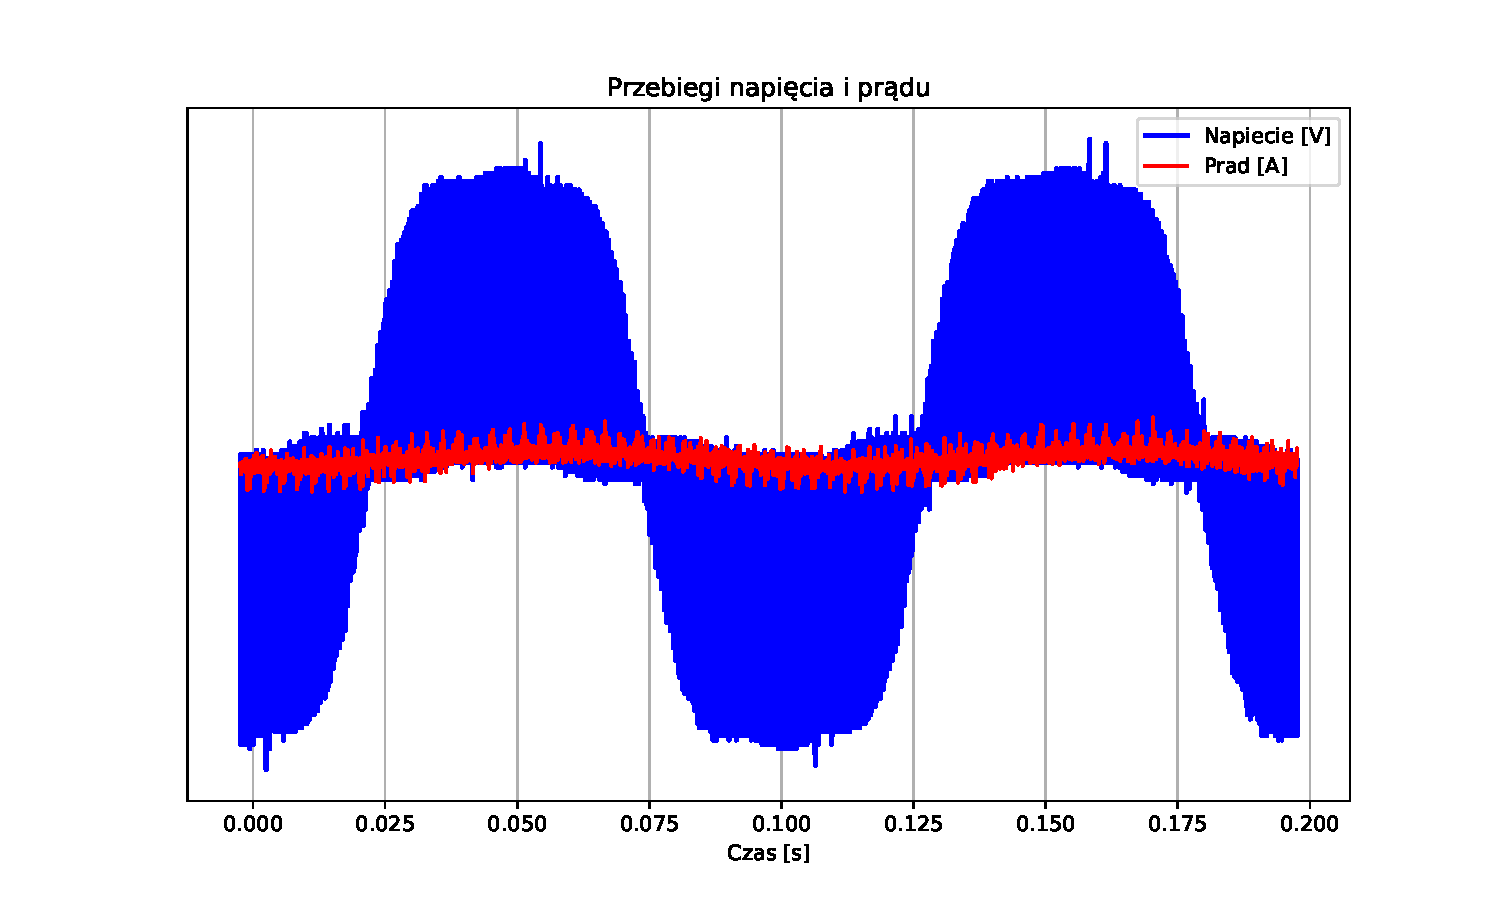
\includegraphics[width=0.8\textwidth]{aun1_microverter_rpm300.pdf}
\caption{Przebieg napięcia oraz prądu na stanowisku Microverter przy prędkości kątowej 300 [RPM]}
\end{figure}

\begin{figure}[H]
\centering
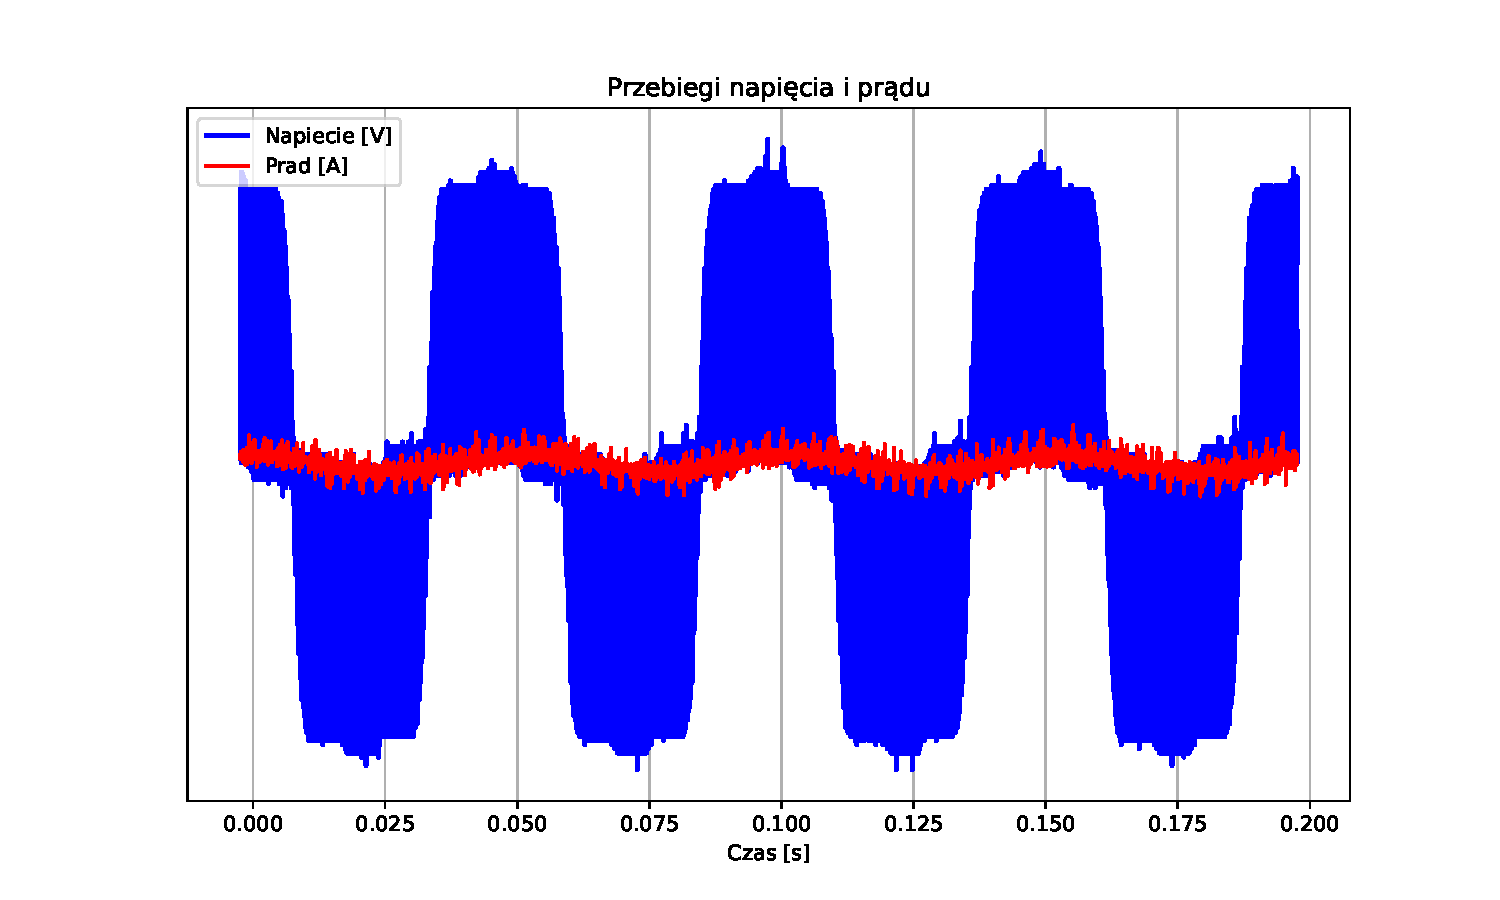
\includegraphics[width=0.8\textwidth]{aun1_microverter_rpm600.pdf}
\caption{Przebieg napięcia oraz prądu na stanowisku Microverter przy prędkości kątowej 600 [RPM]}
\end{figure}

\begin{figure}[H]
\centering
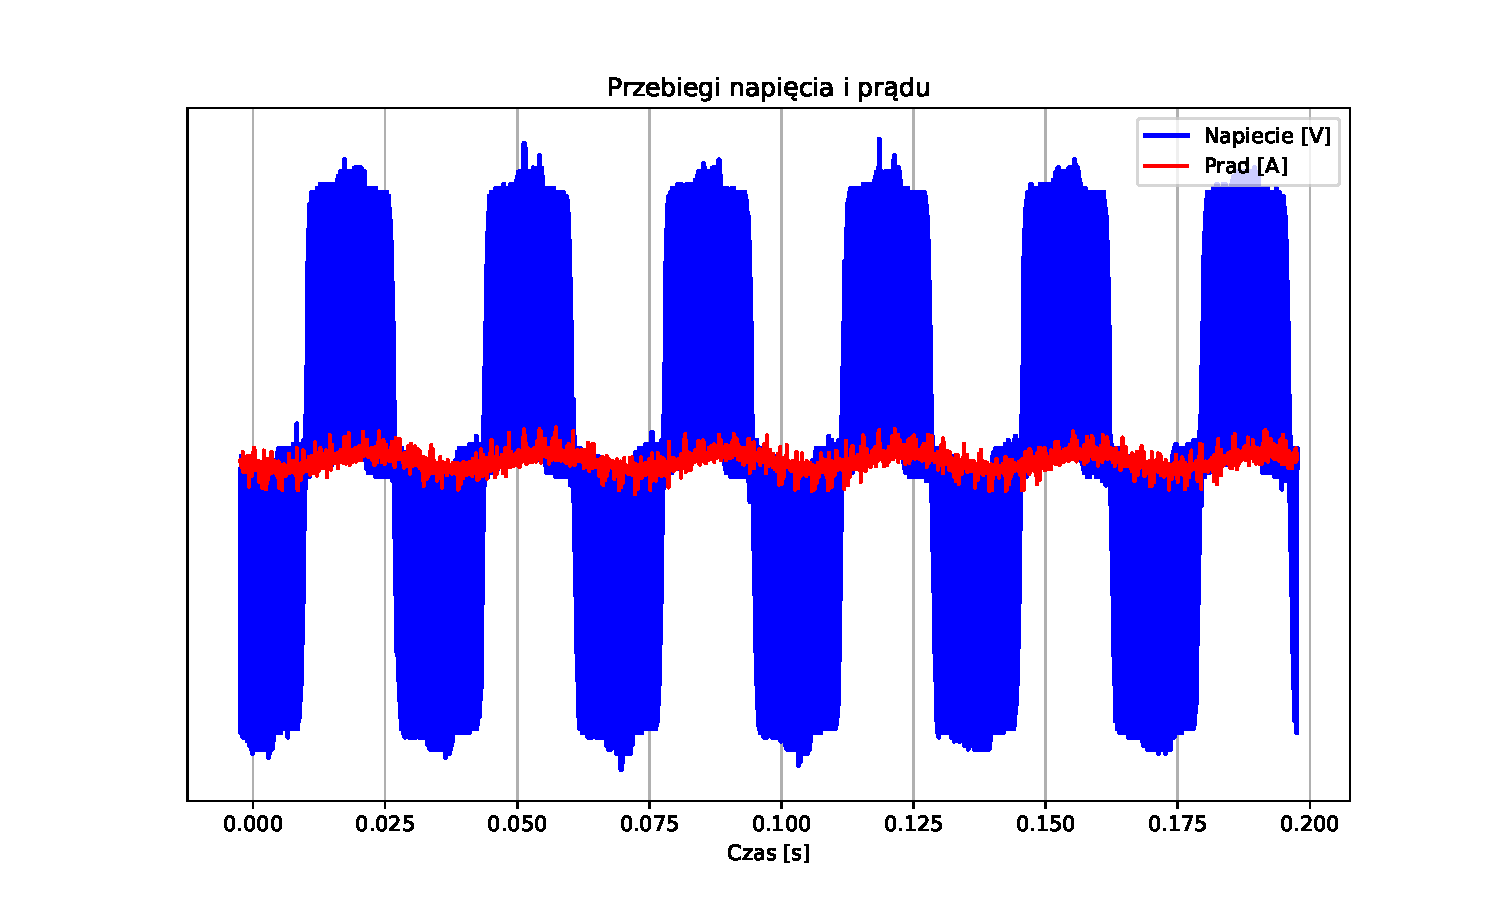
\includegraphics[width=0.8\textwidth]{aun1_microverter_rpm900.pdf}
\caption{Przebieg napięcia oraz prądu na stanowisku Microverter przy prędkości kątowej 900 [RPM]}
\end{figure}

Jak widzimy, napęd Unidrive charakteryzuje się mniejszą częstotliwością i większą amplitudą mierzonych wielkości niż napęd Alspa.\\

Przebiegi napięcia i prądu na stanowisku Unidrive.\\

\begin{figure}[H]
\centering
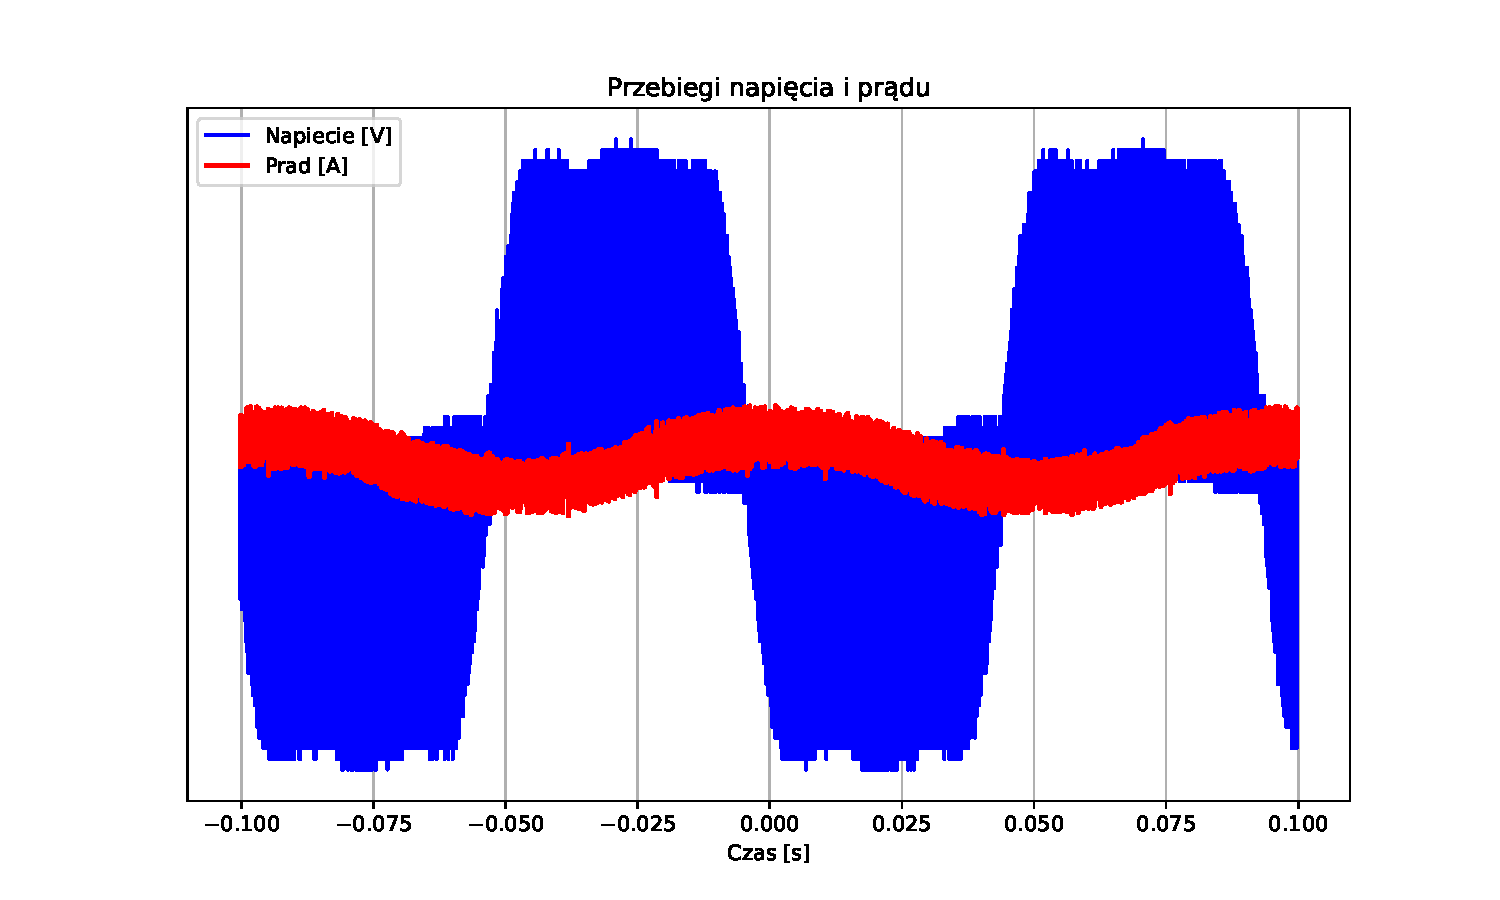
\includegraphics[width=0.8\textwidth]{aun1_unidrive_rpm300.pdf}
\caption{Przebieg napięcia oraz prądu na stanowisku Unidrive przy prędkości kątowej 300 [RPM]}
\end{figure}

\begin{figure}[H]
\centering
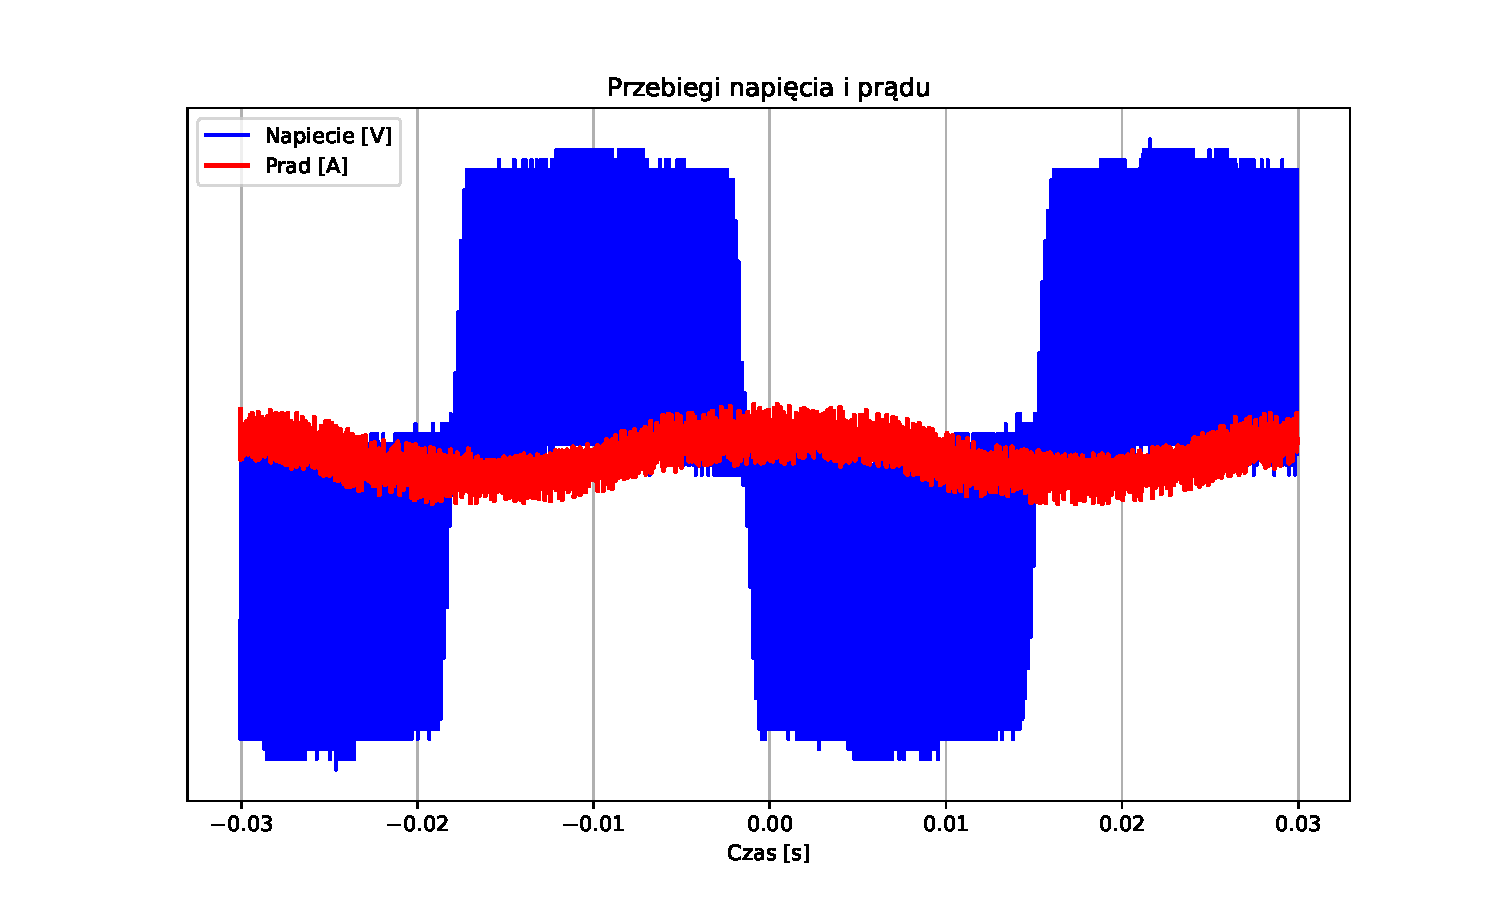
\includegraphics[width=0.8\textwidth]{aun1_unidrive_rpm600.pdf}
\caption{Przebieg napięcia oraz prądu na stanowisku Unidrive przy prędkości kątowej 600 [RPM]}
\end{figure}

\begin{figure}[H]
\centering
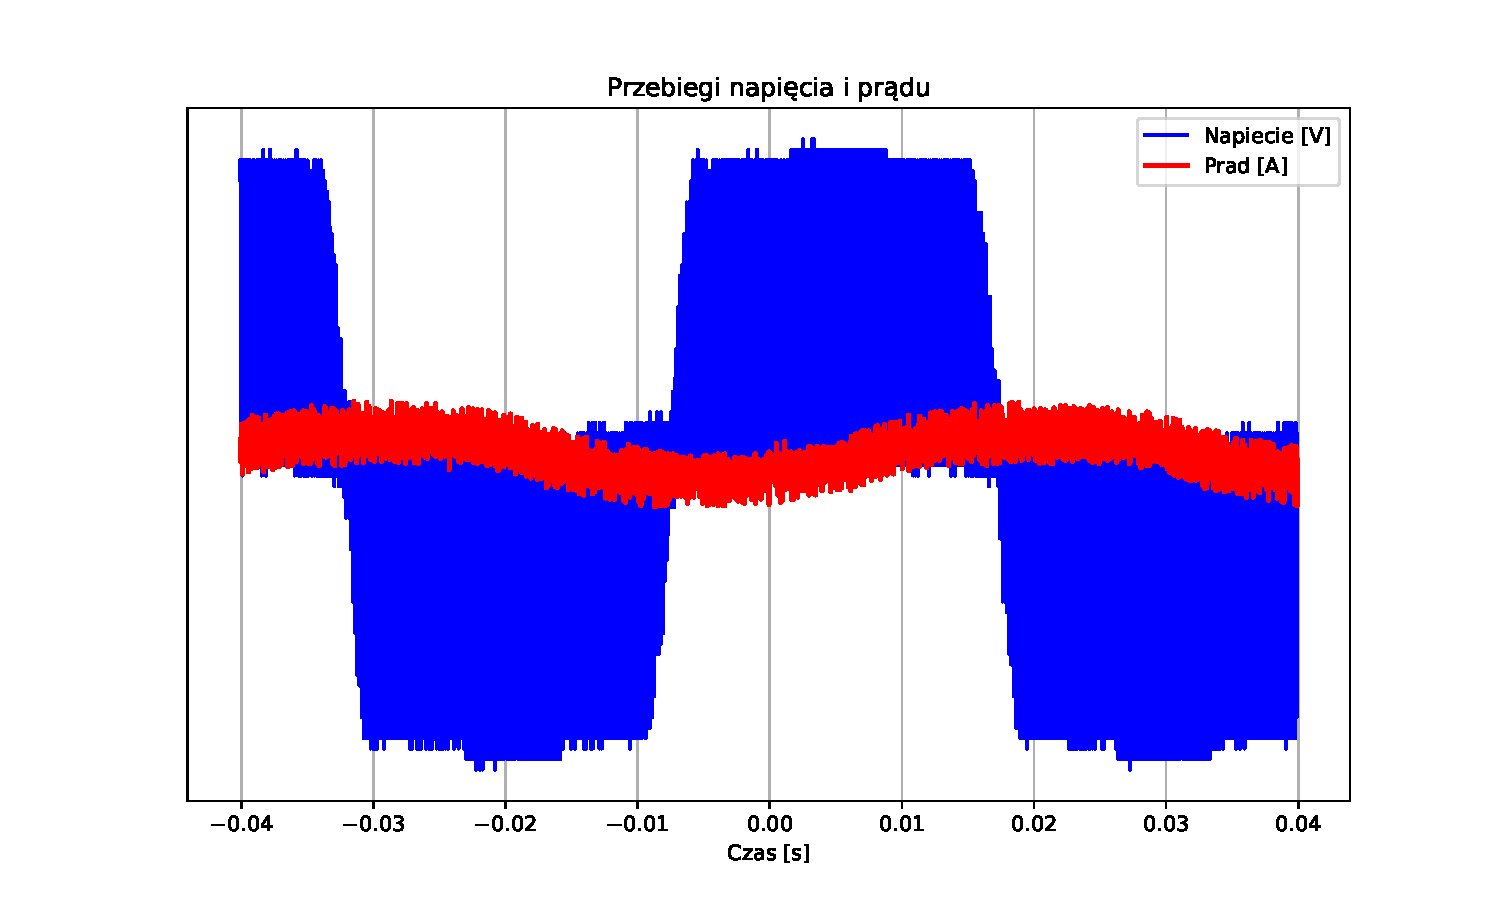
\includegraphics[width=0.8\textwidth]{aun1_unidrive_rpm900.pdf}
\caption{Przebieg napięcia oraz prądu na stanowisku Unidrive przy prędkości kątowej 900 [RPM]}
\end{figure}

Jak widzimy, podobnie do napędu Microverter, napęd Unidrive charakteryzuje się mniejszą częstotliwością i większą amplitudą mierzonych wielkości niż napęd Alspa.\\

\section{Część IV}
\subsection{Analiza działania modelu obwodowego mostka tyrystorowego w LTSpice}
\begin{figure}[H]
    \centering
    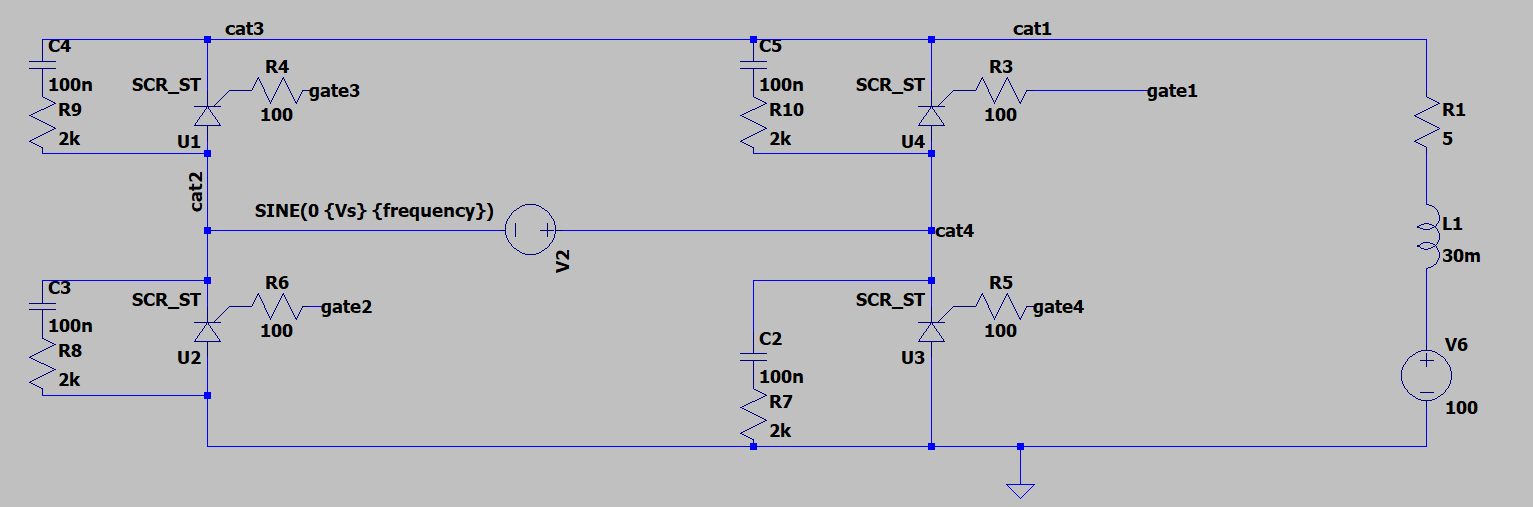
\includegraphics[width=0.85\linewidth]{aun1_fbps-schemat.png}
    \caption{Schemat modelu obwodowego mostka tyrystorowego z tłumieniem}
    \label{fig:fbps-schemat}
\end{figure}
W tej ostatniej części ćwiczenia przeanalizowano działanie modelu obwodowego mostka tyrystorowego wyposażonego w tłumik (Snubber) przedstawionego na schemacie \ref{fig:fbps-schemat}, zrealizowanego w środowisku symulacyjnym LTSpice. Tyrystory, które stanowią kluczowy element układu, zostały użyte do sterowania przepływem prądu przemiennego w obciążeniu poprzez zmianę momentu ich załączenia, wyrażanego jako tzw. kąt wyzwolenia (nazywany dalej fire angle).
Symulacje przeprowadzono przy napięciu sinusoidalnym o amplitudzie \(U_s=230 V\). Do bramek tyrystorów doprowadzano impuls wyzwalający o napięciu 5 V, umożliwiający ich przewodzenie. W tabeli \ref{tab:tabela_fire_angle} przedstawiono zmierzone wartości \(V_{avg}\) oraz \(I_{avg}\) dla kolejnych coraz większych wartości fire angle.
\begin{figure}[H]
    \centering
    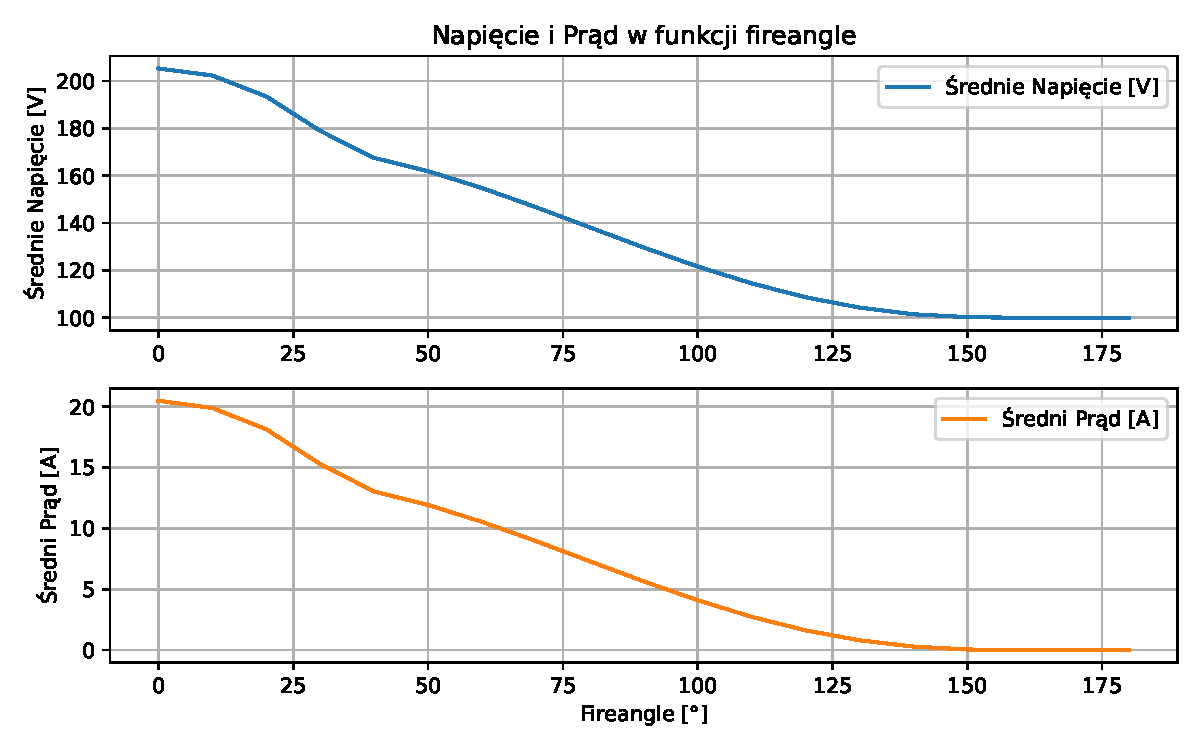
\includegraphics[width=0.7\linewidth]{aun1_tyrystor_fireangle.pdf}
    \caption{Przebieg wartości z tabeli \ref{tab:tabela_fire_angle} w funkcji $Fire angle$}
    \label{fig:wykresIavgVavg}
\end{figure}
\begin{table}[H]
\centering
\caption{Zestawienie wyników pomiarów średniego napięcia i prądu obciążenia}
\begin{tabular}{|c|c|c|}
\hline
\textbf{$Fire\;angle$ [$^\circ$]} & \textbf{$V_{avg}$ [V]} & \textbf{$I_{avg}$ [A]} \\
\hline
0   & 205.325  & 20.4866   \\
10  & 202.341  & 19.8957   \\
20  & 193.498  & 18.1498   \\
30  & 178.976  & 15.2874   \\
40  & 167.536  & 13.0369   \\
50  & 161.921  & 11.9319   \\
60  & 154.814  & 10.5391   \\
70  & 146.744  & 8.9626    \\
80  & 138.205  & 7.2999    \\
90  & 129.687  & 5.6485    \\
100 & 121.659  & 4.1004    \\
110 & 114.543  & 2.7373    \\
120 & 108.679  & 1.6255    \\
130 & 104.304  & 0.8071    \\
140 & 101.483  & 0.2918    \\
150 & 100.264  & 0.0515    \\
160 & 100.001  & 0.0001    \\
170 & 99.9996  & 0.0000    \\
180 & 99.9996  & 0.0000    \\
\hline
\end{tabular}
\label{tab:tabela_fire_angle}
\end{table}


Jak można zaobserwować na danych z tabeli \ref{tab:tabela_fire_angle} oraz wykresie \ref{fig:wykresIavgVavg} średnia wartość napięcia przy wzroście zbiega do 100 V, a średnia wartość prądu do 0 A. Przy 180$^{\circ}$ są to dokładnie takie wartości. Oczywiście jest to efekt działania obwodowego mostka tyrystorowego. Fire angle określa moment przewodzenia tyrystora w mostku względem okresu sygnału. Im wyższa wartość fire angle tym później tyrystor zaczyna przewodzić. Pozwala to nam na sterowanie silnikiem elektrycznym w układzie. Wpływ wartości fire angle na przebiegi napięcia oraz prądu na obciążeniu można zaobserwować na wykresach \ref{fig:aun1_fbps-0} - \ref{fig:aun1_fbps-180}.
\begin{figure}[H]
    \centering
    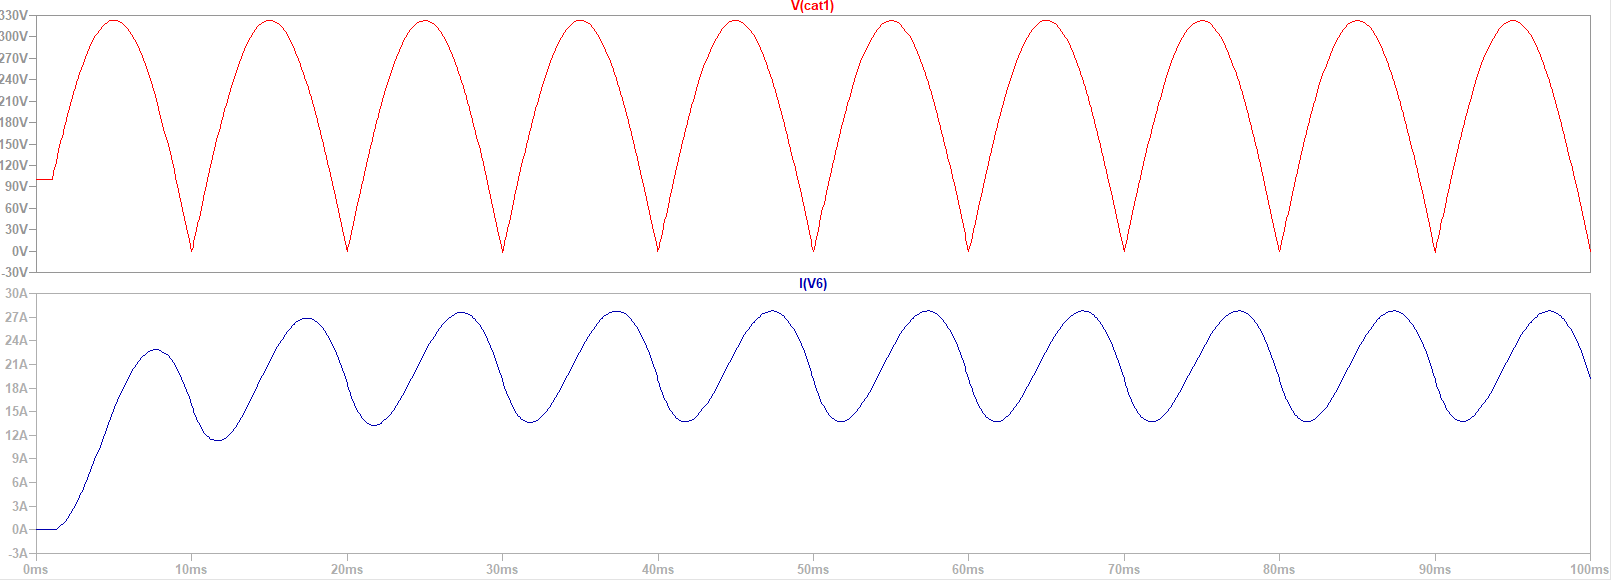
\includegraphics[width=1\linewidth]{aun1_fbps-0.png}
    \caption{Przebieg napięcia oraz prądu dla 0$^{\circ}$}
    \label{fig:aun1_fbps-0}
\end{figure}
\begin{figure}[H]
    \centering
    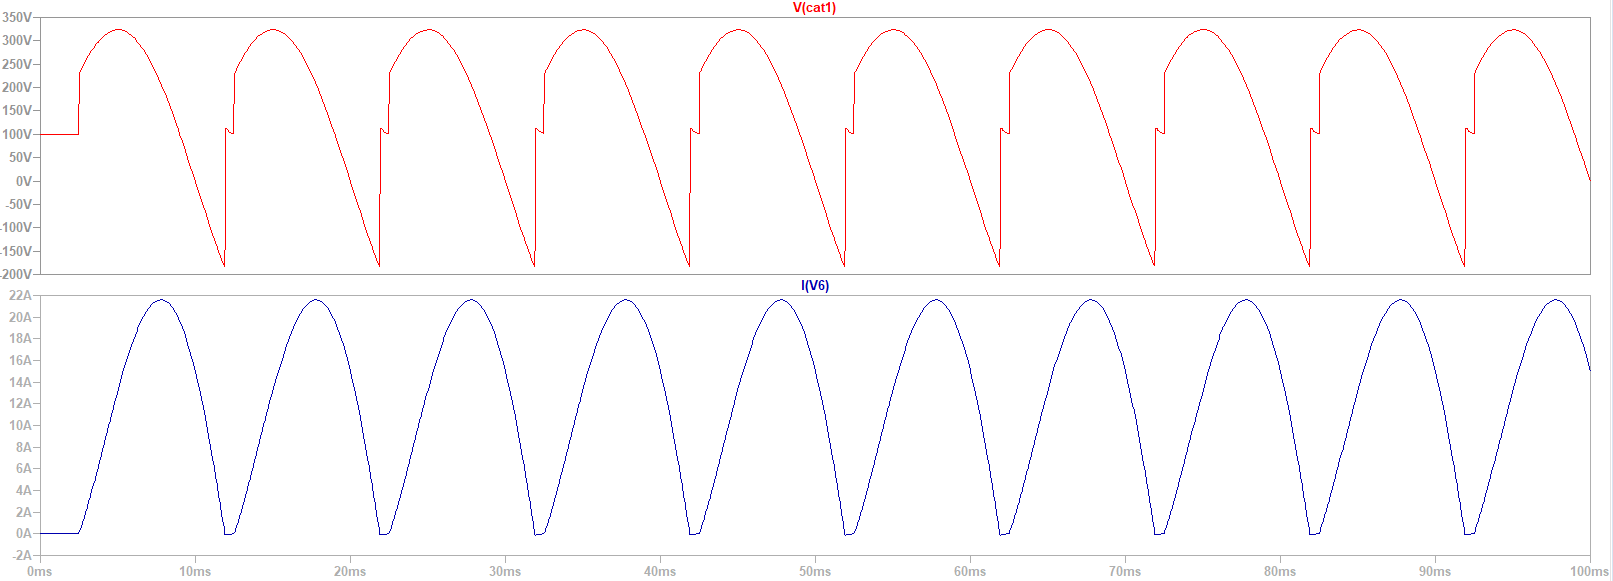
\includegraphics[width=1\linewidth]{aun1_fbps-45.png}
    \caption{Przebieg napięcia oraz prądu dla 45$^{\circ}$}
    \label{fig:aun1_fbps-45}
\end{figure}
\begin{figure}[H]
    \centering
    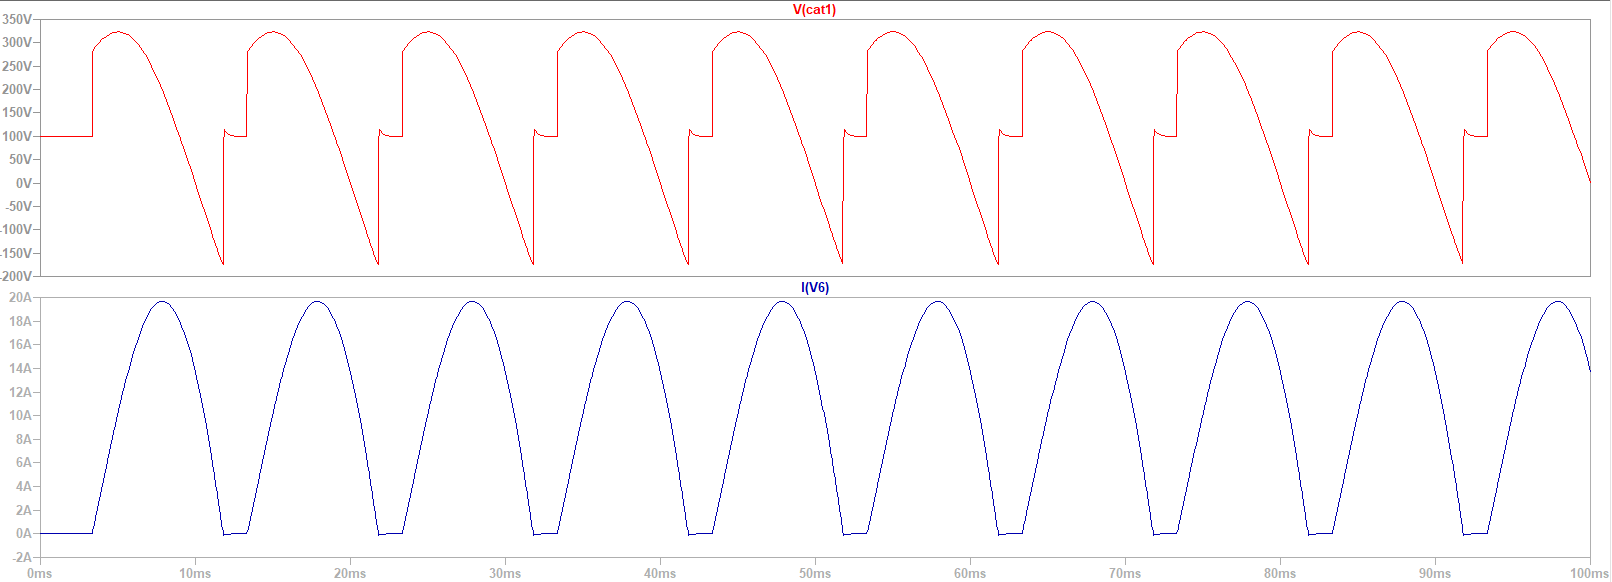
\includegraphics[width=1\linewidth]{aun1_fbps-60.png}
    \caption{Przebieg napięcia oraz prądu dla 60$^{\circ}$}
    \label{fig:aun1_fbps-60}
\end{figure}
\begin{figure}[H]
    \centering
    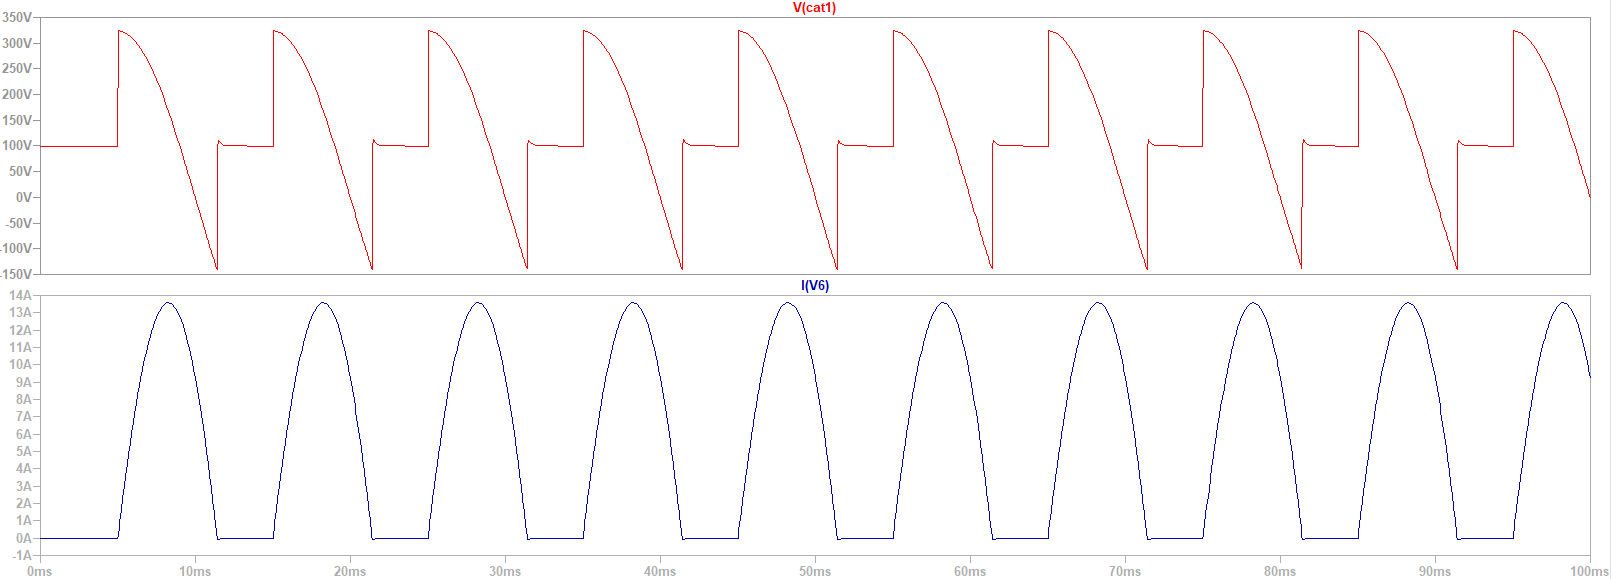
\includegraphics[width=1\linewidth]{aun1_fbps-90.png}
    \caption{Przebieg napięcia oraz prądu dla 90$^{\circ}$}
    \label{fig:aun1_fbps-90}
\end{figure}
\begin{figure}[H]
    \centering
    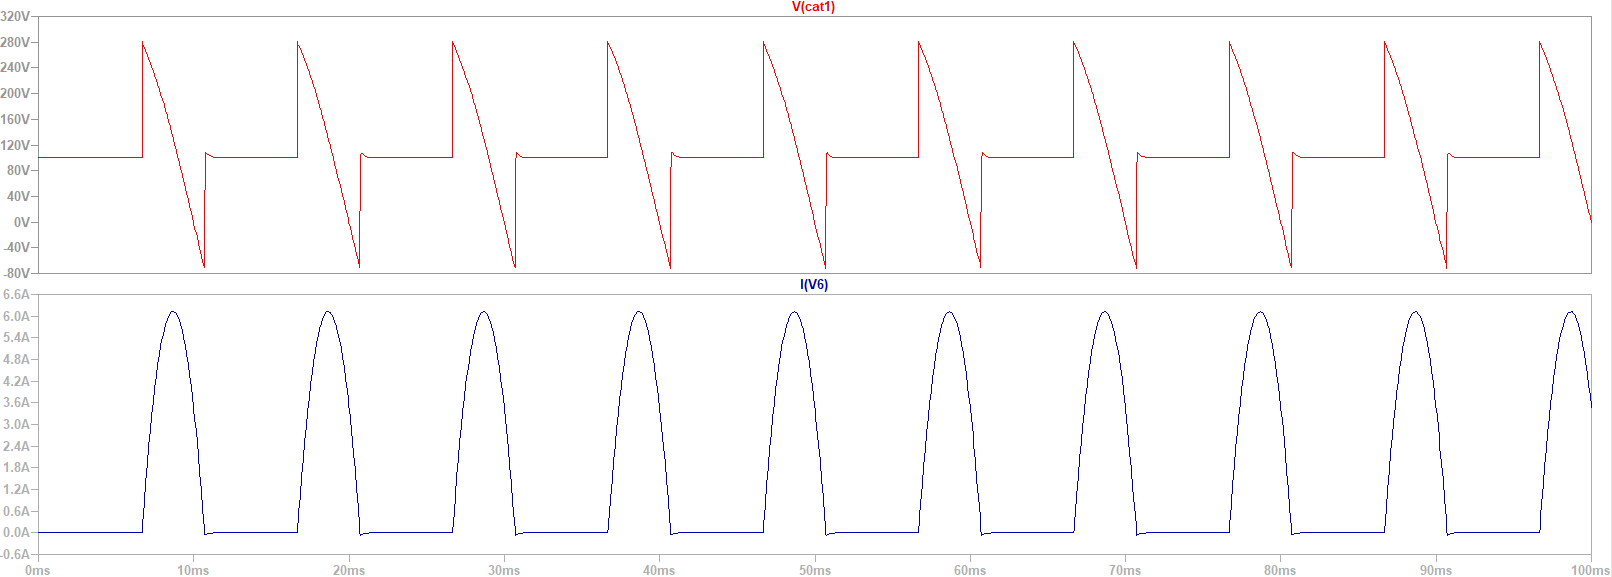
\includegraphics[width=1\linewidth]{aun1_fbps-120.png}
    \caption{Przebieg napięcia oraz prądu dla 90$^{\circ}$}
    \label{fig:aun1_fbps-120}
\end{figure}
\begin{figure}[H]
    \centering
    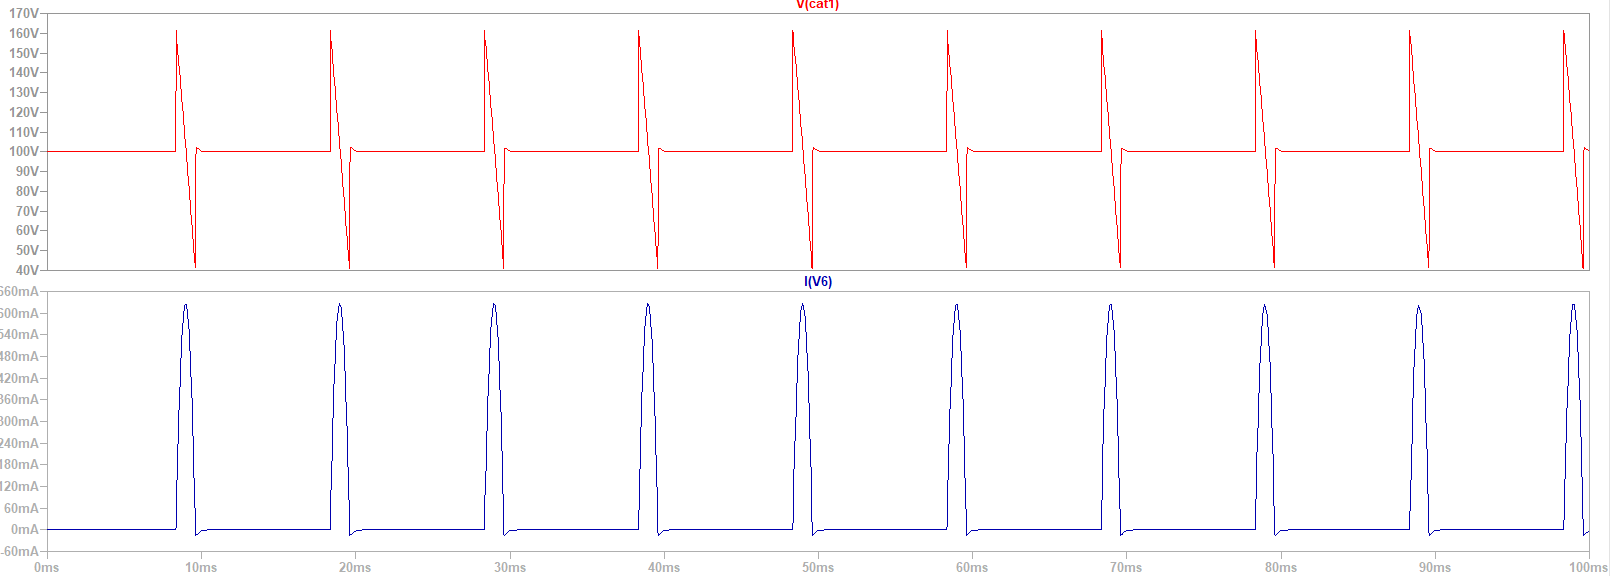
\includegraphics[width=1\linewidth]{aun1_fbps-150.png}
    \caption{Przebieg napięcia oraz prądu dla 150$^{\circ}$}
    \label{fig:aun1_fbps-150}
\end{figure}
\begin{figure}[H]
    \centering
    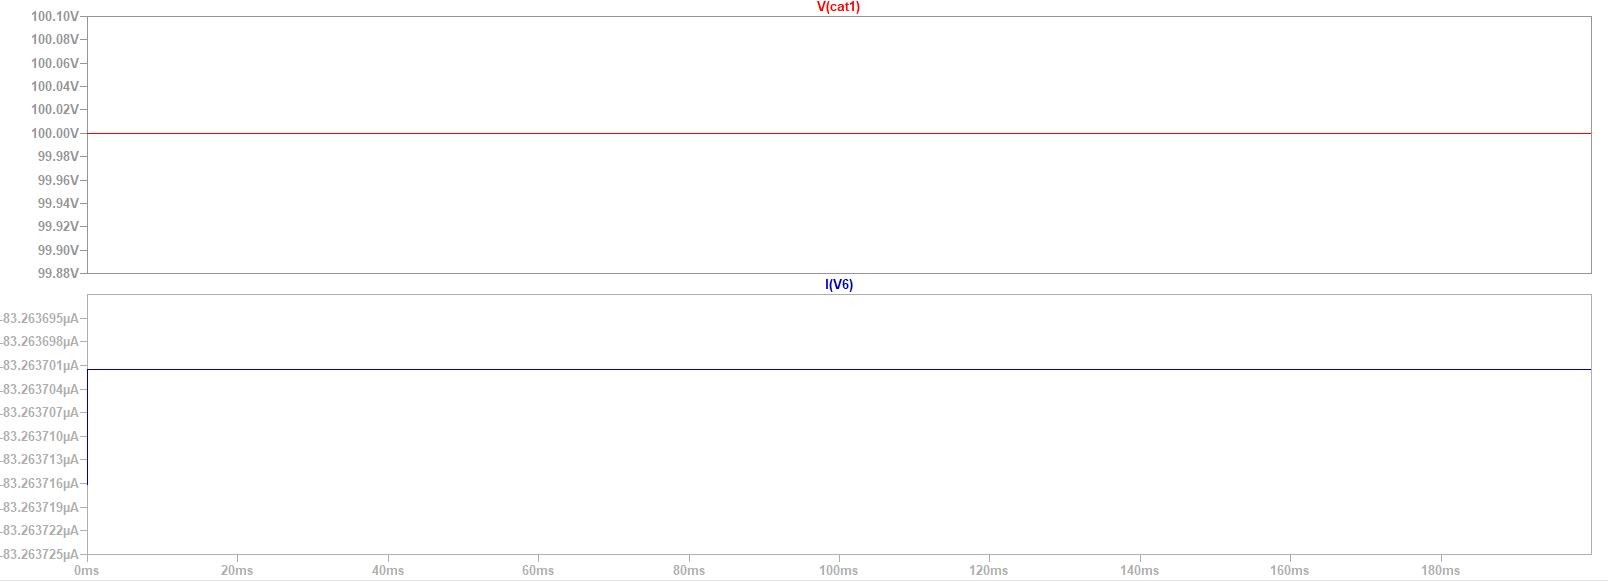
\includegraphics[width=1\linewidth]{aun1_fbps-180.png}
    \caption{Przebieg napięcia oraz prądu dla 180$^{\circ}$}
    \label{fig:aun1_fbps-180}
\end{figure}
Warto zaznaczyć, że do poprawnego działania układu mostka konieczne jest zastosowanie układu tłumiącego procesy przejściowe mostka, które są obecne na schemacie \ref{fig:fbps-schemat}, jednakże gdyby nie zastosowano takiego tłumika, przebiegi wyglądałyby tak jak na wykresie \ref{fig:aun1_fbp-90}. Widać wyraźnie impulsy, które w żaden sposób nie przysłużyłyby się działaniu układy, dlatego wyfiltrowanie ich jest tak kluczowe. 
\begin{figure}[H]
    \centering
    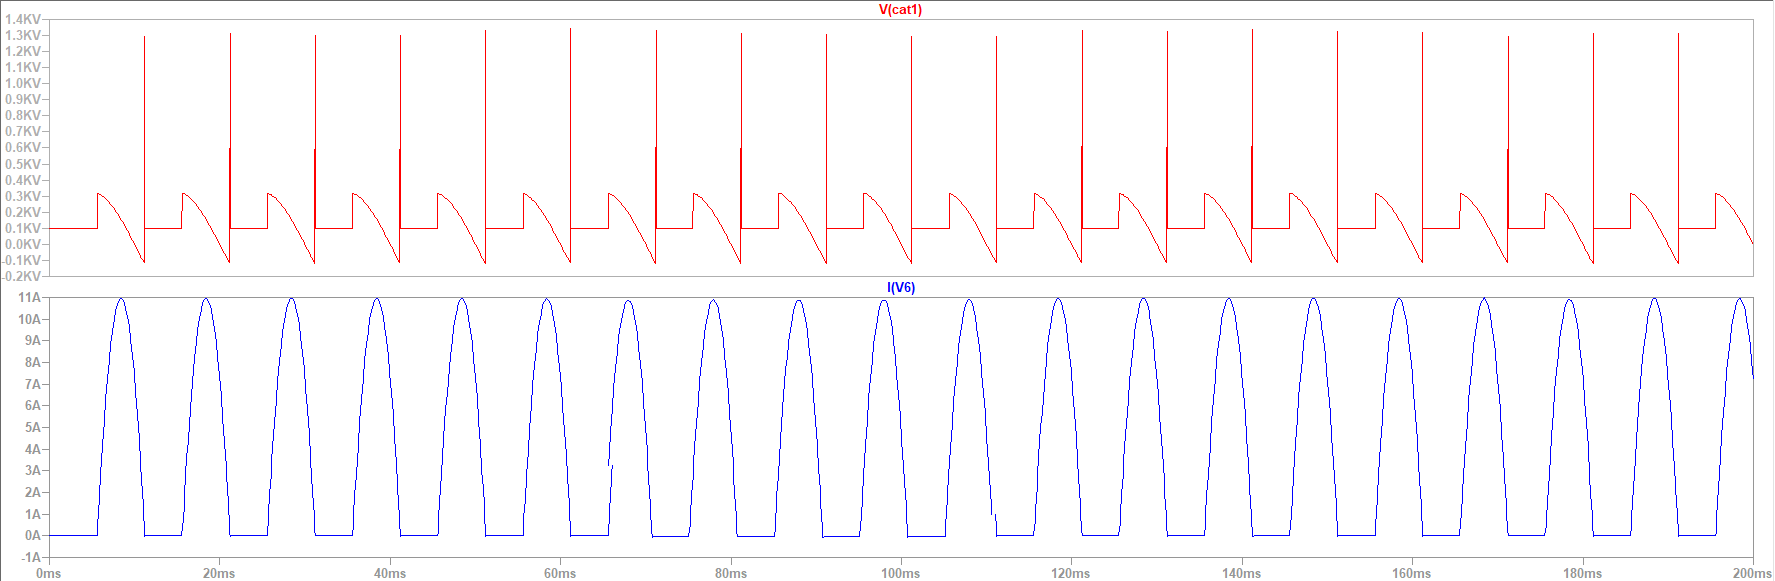
\includegraphics[width=1\linewidth]{aun1_fbp-90.png}
    \caption{Przebiegi napiecia oraz prądu bez elementów tłumiących (bez Snubbera)}
    \label{fig:aun1_fbp-90}
\end{figure}
\subsection{Analiza działania modelu sygnałowego mostka tyrystorowego w Matlab/Simulink}
Następnie zostało zanalizowane działanie modelu sygnałowego mostka tyrystorowego w symulacji simulink wraz z modelem silnika elektrycznego. Sygnałem wejściowym był skok, a na wykresie \ref{fig:smt_VandMC} możemy zaobserwować delikatne opóźnienie transportowe około 200 ms. W stanie przejściowym napięcie silnika oscyluje pomiędzy wartościami dodatnimi, a ujemnymi. Wraz z ustalaniem sygnału i osiągnięciem przez silnik prędkości obrotowej zadanej, napięcie wytraca ujemną część w swoim okresie i jedynie pozostaje dodatnia połówka okresowego sygnału osiągająca w najwyższym punkcie 320 V. Prąd silnika natomiast również charakteryzuje się sygnałem okresowym, który podobnie w procesie przejściowym ustala się na wartości w punkcie najwyższym 20. Jako, że w modelu simulink wartość prądu dla większej przejrzystości wykresu przemnożona jest razy 10, oznacza to że szczytowa wartość sygnału prądu ustala się na poziomie 2 A.
\begin{figure}[H]
    \centering
    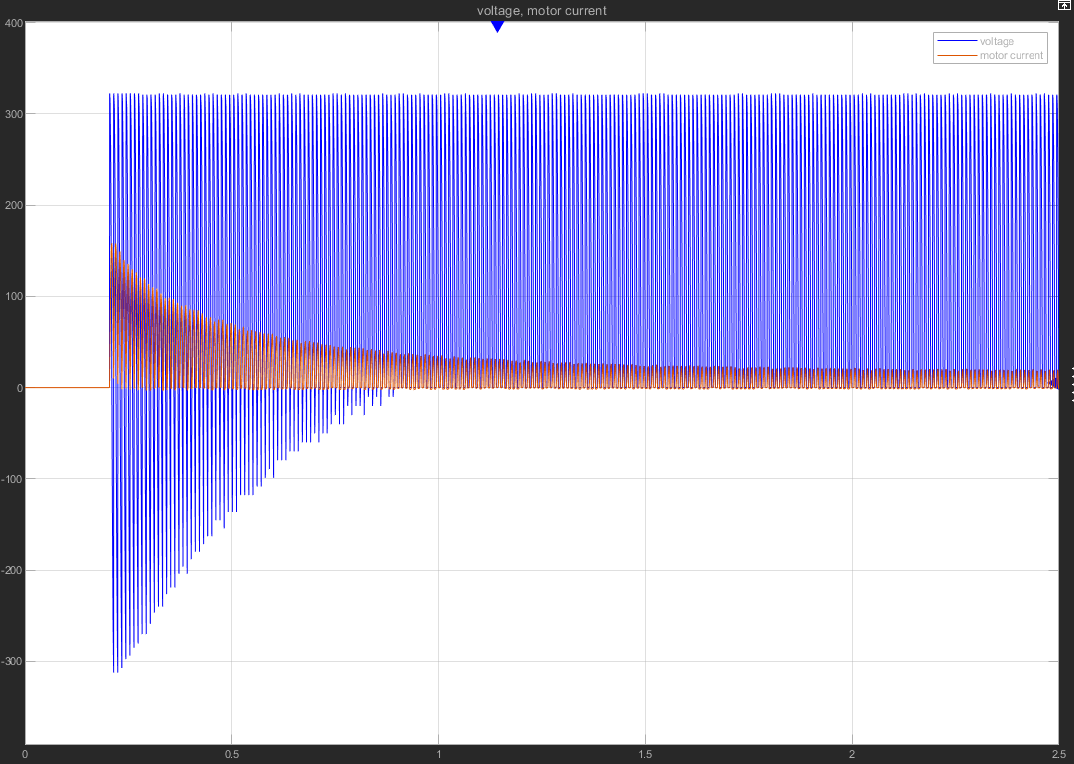
\includegraphics[width=1\linewidth]{aun1_smt_VandMC.png}
    \caption{Przebieg prądu oraz napięcia silnika przy sterowaniu sygnałowym mostkiem tyrystorowym}
    \label{fig:smt_VandMC}
\end{figure}
\begin{figure}[H]
    \centering
    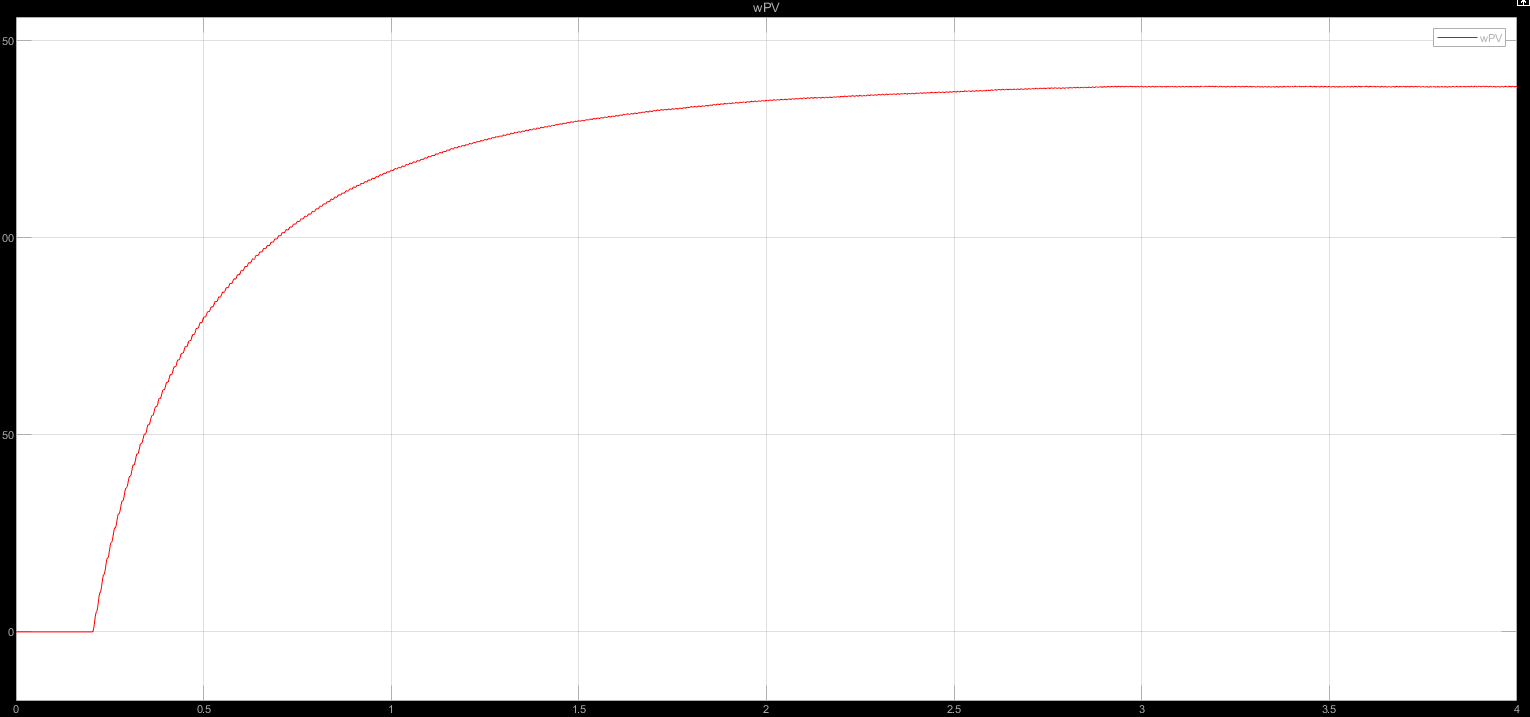
\includegraphics[width=1\linewidth]{aun1_smt_wPV.png}
    \caption{Przebieg prędkości kątowej silnika w rad/s}
    \label{fig:smt_wPV}
\end{figure}
Na wykresie \ref{fig:smt_wPV} Przedstawiony został przebieg prędkości kątowej silnika, udala się ona na wartości około 130 rad/s w czasie 1 sekundy. Warto zaznaczyć, że model wymagał konkretnych zadanych parametrów, aby móc w pełni zasymulować silnik elektryczny. Mają one wpływ na jego dynamikę.
\subsection{Porównanie parametrów pracy napędu z mostkiem tranzystorowym oraz tyrystorowym w procesie sterowania (skokowa zmiana wymuszenia) w Matlab/Simulink}
Porównano sterowanie przy pomocy mostka tranzystorowego oraz tyrystorowego. Obydwa modele sterują silnikiem elektrycznym o takich samych parametrach w modelu simulink. Przebieg prądu silnika na wykresie \ref{fig:tranz_prad} przy sterowaniu mostkiem tranzystorowym ujawnia o wiele większy skok w wartości, ale zarazem o wiele krótszy czas dynamiki przejściowe, z delikatnym podregulowaniem. Zarazem przebieg prędkości zaprezentowany na wykresie \ref{fig:tranz_predkosc}, prędkość nominalna zostaje osiągnięta w o wiele krótszym czasie, wynika to z faktu, że moment obrotowy silnika jest wprost proporcjonalny do prądu płynącego przez uzwojenie. \\
Największą różnicą w obydwu układach mostkowych jest sposób sterowania, w mostku tyrystorowym tak jak widzimy na wykresach \ref{fig:aun1_fbps-0}-\ref{fig:aun1_fbps-180}, modulujemy prąd układu fazowo, zmieniając kąt wyzwolenia co pozwala na dokładne i jawne sterowanie stanem silnika. W przypadku mostka tranzystorowego sterujemy przy pomocy sygnału PWM, dzięki czemu uzyskujemy o wiele większą dynamikę, ale też o wiele większe skoki prądowe w stanach przejściowych. Ich użyteczność zależy od kryteriów ich zastosowania.\\ Jak widzimy na wykresach \ref{fig:smt_VandMC} oraz \ref{fig:smt_wPV} układ z mostkiem tyrystorowym przy takich samych parametrach silnika o wiele wolniej doprowadził silnik do ustalonej nominalnej prędkości, ale z o wiele mniejszym prądem w czasie dynamiki przejściowej.
\begin{figure}[H]
    \centering
    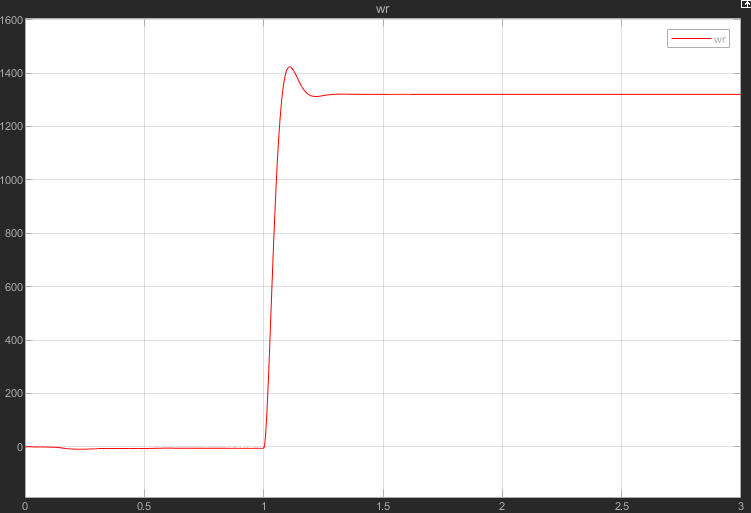
\includegraphics[width=0.9\linewidth]{aun1_tranz_predkosc.png}
    \caption{Przebieg prędkości kątowej silnika przy sterowaniu mostkiem tranzystorowym [rpm]}
    \label{fig:tranz_predkosc}
\end{figure}
\begin{figure}[H]
    \centering
    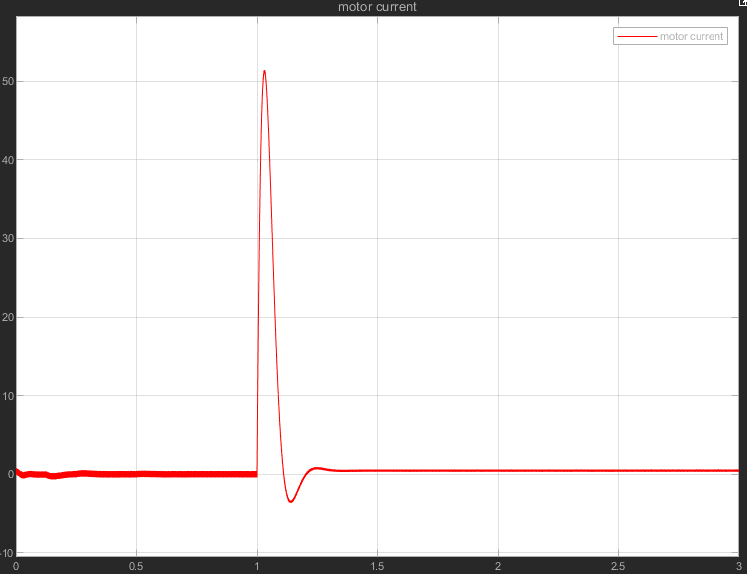
\includegraphics[width=0.9\linewidth]{aun1_tranz_prad.png}
    \caption{Przebieg prądu przy sterowaniu mostkiem tranzystorowym}
    \label{fig:tranz_prad}
\end{figure}

\subsection{Eksperymentalna analiza przebiegów prądu oraz napięcia zasilające silnik napędu DML w różnych stanach pracy (napięcie średnie/obciążenie)}
Pomiary eksperymentalne napędu DML zostały wykonane przez inną grupę i niestety w procesie zostały zapisane jedynie pomiary z oscyloskopu, bez żadnych informacji o aktualnej prędkości obrotowej. Dodatkowo wartości zostały przeskalowane podczas pomiaru, tak aby wysokie wartości napięcia silnika dało się pomierzyć przy pomoc oscyloskopu. 
\begin{figure}[H]
    \centering
    \includegraphics[width=1\linewidth]{aun1_dml2_obciazenie_weak.pdf}
    \caption{Przebieg prądu oraz napięcia silnika przy napędzie DML przy lekkim obciążeniu}
    \label{fig:dml_obciazenie_weak}
\end{figure}
\begin{figure}[H]
    \centering
    \includegraphics[width=1\linewidth]{aun1_dml2_obciazenie_medium.pdf}
    \caption{Przebieg prądu oraz napięcia silnika przy napędzie DML przy średnim obciążeniu}
    \label{fig:dml_obciazenie_medium}
\end{figure}
\begin{figure}[H]
    \centering
    \includegraphics[width=1\linewidth]{aun1_dml2_obciazenie_hard.pdf}
    \caption{Przebieg prądu oraz napięcia silnika przy napędzie DML przy dużym obciążeniu}
    \label{fig:dml_obciazenie_hard}
\end{figure}
Na przebiegu \ref{fig:dml_obciazenie_weak} średnia wartość napięcia \(V_{avg}=58.53\;V\), a średnia wartość prądu \(I_{avg}=0.2496\;A\).\\
Na przebiegu \ref{fig:dml_obciazenie_medium} średnia wartość napięcia \(V_{avg}=175.64\;V\), a średnia wartość prądu \(I_{avg}=0.3359\;A\).\\
Na przebiegu \ref{fig:dml_obciazenie_hard} średnia wartość napięcia \(V_{avg}=235.04\;V\), a średnia wartość prądu \(I_{avg}=0.4125\;A\).\\
Wraz ze wzrostem obciążenia, rośnie średnie napięcie oraz średni prąd.
\end{document}
